% CSC606 Machine Learning -- Phase 2 Final Project Report
% Muhammad Zohaib Chaudhary
% Compile: pdflatex -interaction=nonstopmode final_report.tex   (run twice)
\documentclass[10pt,letterpaper]{article}

\usepackage[T1]{fontenc}
\usepackage{lmodern}
\usepackage[margin=0.9in,top=0.85in,bottom=0.85in]{geometry}
\usepackage{graphicx}
\usepackage{booktabs}
\usepackage{array}
\usepackage{xcolor}
\usepackage{caption}
\usepackage{amsmath}
\usepackage[hidelinks,breaklinks]{hyperref}

\captionsetup{font=small,labelfont=bf,skip=3pt}
\setlength{\parskip}{0.2em}
\setlength{\tabcolsep}{4.0pt}
\renewcommand{\arraystretch}{1.0}
\setlength{\emergencystretch}{3em}
\sloppy
\setlength{\floatsep}{8pt plus 2pt minus 2pt}
\setlength{\textfloatsep}{10pt plus 2pt minus 2pt}
\setlength{\intextsep}{9pt plus 2pt minus 2pt}

% Floats pack densely; otherwise ~20 tables defer and leave half-empty pages.
\renewcommand{\topfraction}{0.92}
\renewcommand{\bottomfraction}{0.80}
\renewcommand{\textfraction}{0.05}
\renewcommand{\floatpagefraction}{0.80}
\setcounter{topnumber}{4}
\setcounter{bottomnumber}{3}
\setcounter{totalnumber}{6}
\setcounter{tocdepth}{1}

\newcommand{\dd}{$\Delta$}
\newcommand{\pmx}{$\pm$}

\title{\vspace{-1.1cm}\textbf{Class Balancing and Calibration for Toxicity Prediction\\ on New Chemical Scaffolds}}
\author{Muhammad Zohaib Chaudhary}
\date{CSC606 Machine Learning --- Phase 2 Final Project Report \quad$\cdot$\quad 25 November 2026}

\begin{document}
\maketitle
\vspace{-0.7cm}

\begin{abstract}
\noindent\small
This project asks which class-balancing methods help a model find more active compounds on
\emph{new chemical scaffolds} while keeping its predicted probabilities reliable. A complete
factorial benchmark of 144 models was fitted and evaluated: three Tox21 assays (NR-AR, NR-AhR,
SR-MMP) $\times$ two split designs (scaffold, random) $\times$ three partition seeds $\times$ two
classifiers (regularised logistic regression, random forest) $\times$ four balancing methods (none,
inverse-frequency class weights, random undersampling to 1:1, SMOTEENN), with 1{,}728 additional
cross-validation fits used for model selection and zero failed configurations. Detection and
probability quality are reported separately and never conflated. Over all 36 paired comparisons per
method, class weighting is the only method that did not systematically cost detection (mean
$\Delta$ average precision $+0.0112$; 6 intervals excluding zero favourably against 2 unfavourably),
while random undersampling ($-0.0216$; 0 / 10) and SMOTEENN ($-0.0329$; 1 / 16) reduced it more
often than they improved it. The one combination with interval-supported gains was class weighting
with the random forest on the scaffold split (mean $\Delta$ AP $+0.0253$ over nine comparisons, 4
favourable and 0 unfavourable intervals, present on two of three assays). Balancing severely
degraded raw probabilities: 84 of 144 raw models score worse on Brier than a constant-prevalence
reference, and all 84 are balanced models. Sigmoid calibration on a separate partition repaired
this for all 144 models without --- and provably without --- changing any ranking metric. Testing on
held-out scaffolds was uniformly harder: average precision fell in 24 of 24 cells and across-seed
variability rose by a factor of 2.43.
\end{abstract}

{\small\vspace{-0.3cm}\tableofcontents}
\vspace{0.2cm}

% ======================================================================
\section{Project Title and Student Information}
% ======================================================================

\noindent
\textbf{Final project title:} Class Balancing and Calibration for Toxicity Prediction on New
Chemical Scaffolds. \quad\textbf{Student:} Muhammad Zohaib Chaudhary. \quad\textbf{Course:} CSC606
Machine Learning, Fall 2026, Phase 2. \quad\textbf{Project type:} individual project, no group
members. \quad\textbf{Deliverables:} this report and the shared Google Colab notebook (final
section, \emph{Google Colab Notebook}, p.~\pageref{sec:colab}).

\textbf{Approved topic.} The Phase 1 proposal set out to test whether balancing the training data
helps models find active compounds with unfamiliar chemical structures, and what balancing does to
the reliability of the predicted probabilities. It specified three Tox21 assays spanning different
degrees of class imbalance, two classifiers, four balancing choices, a primary scaffold-held-out
evaluation with a stratified random split as reference, three fixed seeds, and a separate
calibration partition. The final project carried out exactly that plan: the problem, dataset,
feature representation, classifiers, balancing methods, split designs, seeds, metric set and
evaluation protocol are all as proposed, and the full $3\times2\times3\times2\times4=144$ model grid
was executed to completion.

\subsection{Changes from the proposal}
\label{sec:departures}

Three refinements were made during implementation. \textbf{None changes the problem, the dataset or
the main machine learning approach.}

\begin{enumerate}\setlength{\itemsep}{1pt}
\item \textbf{Execution environment.} The proposal specified Google Colab execution. The 144-model
benchmark was in fact \textbf{executed locally on CPU} (macOS, Python 3.12.14, three parallel worker
processes); the submitted notebook contains the complete implementation and supports Colab
reproduction. The reason is runtime control over 1{,}872 total model fits with content-addressed
caching and checkpoints that survive interruption, which Colab session limits made unreliable.
\item \textbf{RDKit version.} RDKit was \textbf{pinned back from 2026.09.2 to 2025.09.3} before any
data were prepared, because the newer build raised \texttt{RuntimeError: bad any cast} during
Bemis--Murcko scaffold extraction on this host, even for simple valid SMILES. Unexpected runtime
errors now halt preprocessing rather than being recorded as invalid input.
\item \textbf{Calibration implementation.} The sigmoid is fitted with a \textbf{nonnegative-slope
constraint and Platt-smoothed targets} --- an explicit implementation choice. A monotone
non-decreasing map cannot reorder compounds, which is what makes the proposal's rule ``if
calibration preserves the ranking, do not count it as a ranking improvement'' verifiable rather
than merely asserted (Section~\ref{sec:ranking}).
\end{enumerate}

% ======================================================================
\section{Introduction and Problem Significance}
% ======================================================================

\textbf{The machine learning problem.} Each assay is a separate \textbf{binary classification task}.
The input is a molecule encoded as a fixed 2{,}048-dimensional binary vector (a Morgan fingerprint
of radius 2, Section~\ref{sec:features}); the target is the recorded assay outcome, 1 for active and
0 for inactive. The application domain is computational toxicology, specifically the triage step
that decides which compounds from a large library are sent for laboratory testing. The defining
characteristic of the data is \textbf{class imbalance}: actives are 4.28\% of cleaned NR-AR, 11.91\%
of NR-AhR and 15.92\% of SR-MMP --- roughly 1 active in 23, 1 in 8 and 1 in 6 compounds. A model
that predicts ``inactive'' for everything achieves 95.7\% accuracy on NR-AR while being useless for
its purpose, so accuracy is not reported anywhere in this project.

\textbf{Why it matters.} Two distinct things can go wrong, and resampling the training data ---
the standard response to imbalance --- addresses only one of them. \emph{Detection:} a screening
campaign has a fixed budget, so what matters is how many true actives appear in the top-ranked
fraction, measured here by average precision and by precision and recall inside a fixed top-10\%
budget identical for every method. \emph{Reliability of the predicted probability:} downstream
decisions use the predicted number, not just the ordering --- if a model assigns 100 compounds a
probability near 0.20, about 20 should be active for that number to mean anything. Balancing
deliberately distorts the training class ratio, so it affects this quantity directly and separably
from any effect on ranking. \emph{New scaffolds:} a random split largely asks about compounds whose
chemical core the model has already seen, whereas real screening asks about new chemistry, which is
why holding out whole Bemis--Murcko scaffold groups is the primary design here and the random split
is kept only as a reference.

\textbf{Research questions.} \textbf{RQ1 (detection)} --- do class weights, random undersampling
or SMOTEENN increase the number of actives found within a fixed screening budget, relative to no
balancing, on the same assay, split, seed, classifier and calibration state? \textbf{RQ2
(probability quality)} --- what does each method do to Brier score, log loss and the reliability
curve, and how much does sigmoid calibration on a separate partition undo? \textbf{RQ3 (scaffold
generalisation)} --- does any detection benefit survive when test compounds come from scaffold groups
absent from training, and how much do performance and stability change? \textbf{RQ4 (mechanism)} ---
can the behaviour be explained by what each method does to the training set and the predicted score
distribution, rather than only reported as a number?

\textbf{Scope of the claim.} Tox21 assay activity is an \textbf{experimental endpoint}. An active
result in one of these assays is \emph{not} a determination that a chemical is harmful to people.
Every conclusion here concerns model performance, probability calibration, and the limits of this
evaluation --- nothing further.

\subsection{Conventions used throughout this report}
\label{sec:conventions}

\begin{enumerate}\setlength{\itemsep}{1pt}
\item \textbf{Sign convention.} Every delta is \emph{balancing method minus the unbalanced
\texttt{none} baseline}, within the same assay, split kind, seed, classifier and calibration state.
For \textbf{average precision, ROC AUC, precision and recall a positive delta is favourable}; for
\textbf{Brier score and log loss a negative delta is favourable}, because both are losses.
\item \textbf{Intervals are descriptive, and no significance is claimed.} All intervals are 95\%
percentile intervals from 1{,}000 paired bootstrap replicates drawn \emph{conditional on the
already-fitted models and the current test partition}. They capture neither retraining nor split
uncertainty and are not adjusted for the large number of comparisons made here. No comparison in
this report is described as statistically significant and no hypothesis test or $p$-value is
computed anywhere; an interval that excludes zero is described as exactly that, in this one test
partition.
\item \textbf{Three seeds are not independent replication.} The \pmx{} values are standard
deviations over the three partition seeds, which draw \emph{overlapping} test sets from the same
cleaned table. They are split and fit variation, not standard errors, and establish nothing about
reproducibility across datasets.
\item \textbf{Exploratory labelling.} Per the pre-registered rule, any subset with fewer than 20
positive compounds is \emph{exploratory} and is labelled so wherever it appears.
\end{enumerate}

% ======================================================================
\section{Literature Review}
% ======================================================================

\textbf{Imbalance corrections in Tox21 modelling.} Idakwo et al.~[1] studied highly imbalanced Tox21
assays with random forests, comparing random undersampling, SMOTE and SMOTEENN, and --- unusually
for this literature --- reported Brier scores alongside classification measures. SMOTEENN performed
well overall there, which is the direct reason SMOTEENN rather than plain SMOTE is in this project's
method set; their curation, bagging design, descriptors and tuning differ, so their numbers are
motivation, not a baseline this report can be scored against. Santiago-Gonzalez et al.~[2] compared
balancing approaches across ten Tox21 bioassays, six molecular representations and five classifiers
--- a far wider sweep of \emph{methods} than attempted here. The present work deliberately narrows
the method axis and spends the saved effort on the \emph{evaluation} axis: a held-out-scaffold
design, a separate calibration partition, and paired within-partition uncertainty for every
comparison. \emph{Verification:} [2] is verified as bibliographic metadata and publisher abstract
only; the full text is paywalled and was not purchased, so no specific methodological claim about it
is asserted here.

\textbf{The cost of imbalance correction to predicted probabilities.} Van den Goorbergh et al.~[3]
is the closest methodological antecedent for the second half of the research question. Using
simulations and a clinical case study, they found that imbalance corrections applied to logistic
regression could badly distort predicted risks while leaving discrimination essentially unchanged
--- the correction moved the probabilities without improving the ordering. Their evidence comes from
clinical risk prediction with a handful of covariates, not from 2{,}048-bit chemical fingerprints or
tree ensembles, so the direction cannot simply be assumed to carry over.
Sections~\ref{sec:detect} and \ref{sec:prob} test both halves of that claim here, for two model
families rather than one.

\textbf{Leakage-audited benchmarking and scaffold splits.} The ToxBench study~[4] is the closest
contemporary evaluation framework: a leakage-audited multi-task predictive-toxicology benchmark
comparing random and scaffold splits, examining calibration and uncertainty, and including
nearest-neighbour applicability-domain analysis. This project adopts that style of evaluation to
answer a different question --- not ``how well do models do on this benchmark'' but ``what does the
choice of balancing method cost or buy, under exactly the same partition and budget''.
\emph{Verification:} [4] is verified as bibliographic metadata and publisher abstract only; it is an
early-access accepted manuscript and the full PDF fetch timed out. \textbf{The proposal's specific
assertion that that study uses class weighting for its tree models could not be independently
verified from the accessible article text and is not asserted as confirmed anywhere in this report.}

\textbf{Data, libraries and reference implementations.} The dataset is the public Tox21 CSV linked
by DeepChem's official loader~[5], read directly but with this project's own documented
preprocessing rather than DeepChem's default label transformer or built-in benchmark split, so that
every cleaning decision is traceable. RDKit~[6] performs parsing, standardisation, canonical
identity and fingerprint generation; imbalanced-learn~[7] provides SMOTEENN; and the scikit-learn
probability-calibration user guide~[8] is the reference for the calibration design, in particular
the requirement that calibration data be disjoint from the data used to fit the model.

\textbf{How this project relates, extends and differs.} It \emph{relates} to [1], [2] and [4]
through the dataset family, the balancing families and the calibration concern. It \emph{extends}
them by reporting detection and probability quality as two separate results for the same 144 models,
under a pre-registered rule that a rank-preserving calibration map may never be credited with a
ranking gain --- and then \emph{verifying}, rather than assuming, that the map is rank-preserving
(Section~\ref{sec:ranking}). It \emph{differs} in being strictly paired: every method is compared
with the unbalanced baseline on the same assay, partition, seed, classifier and calibration state,
with a cluster bootstrap that resamples whole scaffold groups on scaffold partitions. The question
is the \emph{difference}, so the absolute numbers here are not intended to compete with published
leaderboard values.

% ======================================================================
\section{Data Description and Preprocessing}
% ======================================================================

\textbf{Source, size and target.} The input is the public compressed Tox21 CSV linked by DeepChem's
official loader~[5]; the downloaded bytes, their SHA-256, the UTC download timestamp, the column
list and the record count are retained in \texttt{data/raw/source.json}. The executed download
contains \textbf{7{,}831 records}, each a SMILES string plus twelve assay-label columns. Three
assays were selected in the proposal to span a useful range of imbalance across nuclear-receptor and
stress-response biology: \textbf{NR-AR} (androgen receptor), \textbf{NR-AhR} (aryl hydrocarbon
receptor) and \textbf{SR-MMP} (mitochondrial membrane potential). The target is the binary activity
call for a single assay; each assay is a separate task.

\subsection{Data issues addressed}

Four real data problems were handled, under rules fixed before any split was drawn.

\begin{itemize}\setlength{\itemsep}{1pt}
\item \textbf{Invalid and inorganic structures.} RDKit parses each SMILES and applies
\texttt{rdMolStandardize.Cleanup}. Fragments containing at least one carbon atom are eligible; the
retained fragment has greatest heavy-atom count, then greatest atom count, with ascending canonical
isomeric SMILES breaking ties; \texttt{Uncharger} is then applied and the result sanitised. Of the
7{,}831 records, \textbf{8 failed SMILES parsing} and \textbf{80 contained no carbon-bearing
fragment}, leaving \textbf{7{,}743 structurally eligible records}. Every exclusion is logged.
\item \textbf{Duplicate structures.} Canonical isomeric SMILES defines identity and its SHA-256 is
the structure ID; stereoisomers remain distinct. The 7{,}743 eligible records collapse to
\textbf{7{,}524 unique standardised structures}, and within an assay duplicates with consistent
labels are merged into one record.
\item \textbf{Conflicting labels.} A structure whose duplicate records disagree about activity in an
assay is removed from \emph{that assay entirely} (7--10 structures per assay). It is not silently
resolved by majority vote.
\item \textbf{Missing labels.} A missing assay label excludes its record from \emph{that assay
only}, and is never treated as an inactive result. This is why the three assays differ in size.
\end{itemize}

There are no missing \emph{feature} values to impute --- the fingerprint is computed
deterministically from the structure --- no categorical variables to encode, and no outliers in the
usual numeric sense, because every feature is a bit.

\begin{table}[!htbp]
\centering
\footnotesize
\caption{Per-assay cleaning accounting, from 7{,}831 raw records
(\texttt{data/audit/assay\_counts.csv}). ``Labels'' is the count of records with an observed label
for that assay; ``Invalid'' counts rows dropped for unparseable or non-organic structures;
``Conflict'' counts structures removed for contradictory labels; ``Dups'' counts duplicate rows
merged.}
\label{tab:counts}
\begin{tabular}{@{}lrrrrrrrrr@{}}
\toprule
Assay & Labels & Pos. & Missing & Invalid & Conflict & Dups & Clean $n$ & Clean pos. & Prevalence \\
\midrule
NR-AR  & 7{,}265 & 309 & 566 & 87 & 8 & 204 & 6{,}957 & 298 & 0.0428 \\
NR-AhR & 6{,}549 & 768 & 1{,}282 & 82 & 10 & 168 & 6{,}278 & 748 & 0.1191 \\
SR-MMP & 5{,}810 & 918 & 2{,}021 & 70 & 7 & 145 & 5{,}578 & 888 & 0.1592 \\
\bottomrule
\end{tabular}
\end{table}

\subsection{Feature engineering, and why no further preprocessing}
\label{sec:features}

Every valid unique structure receives a \textbf{binary Morgan fingerprint of radius 2 with 2{,}048
bits and no chirality} (the ECFP4-like setting named in the proposal); each bit records the presence
of a circular substructure environment around some atom, up to two bonds out. This representation is
used because it is standard for this class of structure--activity problem, because it is fixed and
deterministic so that differences between runs are attributable to the balancing method rather than
the features, and because it requires \emph{no learned preprocessing} --- which removes an entire
category of leakage risk, since there is no scaler or decomposition that could be fitted outside the
training partition.

No normalisation is applied: the features are already on a common $\{0,1\}$ scale, and scaling binary
indicators would change neither the logistic decision-boundary family nor the forest's split points.
No feature selection is applied either: $L_2$ regularisation in the logistic model and $\sqrt{p}$
feature subsampling in the forest handle 2{,}048 columns directly, and selecting features globally
would be another opportunity for information to cross partition boundaries. Fingerprints are stored
as \texttt{uint8} and cast to \texttt{float32} before any SMOTE operation, since synthetic
interpolation produces non-integer values.

\subsection{Training/calibration/test strategy and leakage avoidance}

Each assay is split independently into approximately \textbf{60\% training, 20\% calibration, 20\%
test} under three pre-registered seeds (17, 42, 2026). The three-way split exists because
calibration must be fitted on data disjoint from both model fitting and final evaluation~[8];
collapsing it into two parts would either contaminate the calibration map with training data or
contaminate the test estimate with calibration data.

The \textbf{random design} uses two successive stratified splits: hold out 40\%, then divide that
holdout equally. The \textbf{scaffold design} (primary) identifies groups by non-stereochemical
Bemis--Murcko scaffold, with every acyclic structure in a single \texttt{\_\_EMPTY\_\_} group; unique
scaffold names are sorted, sizes multiplied by seeded uniform priorities in $[0.5,1.5]$, and groups
processed in decreasing priority order and allocated to the partition with the largest remaining
absolute capacity against the 60/20/20 targets. \textbf{Scaffold allocation uses only scaffold
membership and group size --- never activity labels}; no compound is discarded and no group is ever
split across partitions.

\textbf{Leakage controls.} Partition isolation was verified on all 18 manifests: zero structure
overlap between training, calibration and test in every case, and for the scaffold design, zero
scaffold overlap as well. Under random splitting, scaffold overlap between training and test is
expected by construction and is quantified at 146--224 shared groups per partition. Test labels are
used for evaluation only, and neither the calibration nor the test partition informed any
hyperparameter choice (Section~\ref{sec:training}).

\begin{table}[!htbp]
\centering
\footnotesize
\caption{Realised partitions (\texttt{partitions/partition\_summary.csv}). Sizes are fixed by the
design; test positives and test prevalence are given as min--max over the three seeds. ``Max dev.''
is the largest deviation of any of the three realised fractions from its 60/20/20 target, in
percentage points.}
\label{tab:partitions}
\begin{tabular}{@{}llrrrccr@{}}
\toprule
Assay & Split & Train $n$ & Calib.\ $n$ & Test $n$ & Test positives & Test prevalence & Max dev.\ (pp) \\
\midrule
NR-AR  & random   & 4{,}174 & 1{,}391 & 1{,}392 & 60--60   & 0.0431--0.0431 & 0.0086 \\
NR-AR  & scaffold & 4{,}174 & 1{,}392 & 1{,}391 & 62--96   & 0.0446--0.0690 & 0.0086 \\
NR-AhR & random   & 3{,}766 & 1{,}256 & 1{,}256 & 149--150 & 0.1186--0.1194 & 0.0127 \\
NR-AhR & scaffold & 3{,}767 & 1{,}256 & 1{,}255 & 170--208 & 0.1355--0.1657 & 0.0096 \\
SR-MMP & random   & 3{,}346 & 1{,}116 & 1{,}116 & 177--178 & 0.1586--0.1595 & 0.0143 \\
SR-MMP & scaffold & 3{,}347 & 1{,}116 & 1{,}115 & 220--238 & 0.1973--0.2135 & 0.0108 \\
\bottomrule
\end{tabular}
\end{table}

Realised fractions land within \textbf{0.015 percentage points} of the requested 60/20/20 in all 18
partitions. Because scaffold allocation is label-independent, scaffold partition prevalence is free
to drift, and it does: the NR-AhR scaffold calibration partition ranges from 13.69\% to 18.71\%
active across seeds, and the NR-AR scaffold test partition from 4.46\% to 6.90\%, while the
corresponding random partitions are effectively fixed. \textbf{Test prevalence therefore differs
between the two split kinds, and because average precision has prevalence as its floor, average
precision is not directly comparable across split kinds without correction.}
Section~\ref{sec:scaffvrand} reports a prevalence-normalised ratio for exactly this reason.

\subsection{The scaffold-split caveat}
\label{sec:scaffcaveat}

This is the most important structural limitation of the primary experiment, and it is stated here
rather than buried in the limitations. Under the fixed, label-independent allocation rule, the two
giant scaffold groups --- \texttt{\_\_EMPTY\_\_} (every acyclic compound, pooled into one group by
design) and plain benzene \texttt{c1ccccc1} --- are the first groups placed and \textbf{always land
in training}, for every assay and every seed.

\begin{table}[!htbp]
\centering
\footnotesize
\caption{The two giant scaffold groups, derived from the per-assay scaffold partition manifests.
Both are allocated to training for every assay and all three seeds. ``Pool'' is the number of
compounds remaining once those two groups are removed.}
\label{tab:giant}
\begin{tabular}{@{}lrrrrrrr@{}}
\toprule
Assay & Groups & \texttt{\_\_EMPTY\_\_} & Benzene & \% of assay & \% of train & Pool & Test \% of pool \\
\midrule
NR-AR  & 2{,}104 & 1{,}559 & 1{,}359 & 41.9\% & 69.9\% & 4{,}039 & 34.4\% \\
NR-AhR & 1{,}878 & 1{,}496 & 1{,}230 & 43.4\% & 72.4\% & 3{,}552 & 35.3\% \\
SR-MMP & 1{,}625 & 1{,}354 & 1{,}142 & 44.7\% & 74.6\% & 3{,}082 & 36.2\% \\
\bottomrule
\end{tabular}
\end{table}

The consequence is explicit: \textbf{the scaffold test set is the remaining scaffold distribution,
not a uniform draw over all scaffold groups.} Between 41.9\% and 44.7\% of each assay's compounds sit
in two groups guaranteed to be training data, and those two groups make up 69.9--74.6\% of each
training partition. The held-out 20\% comes from the other ${\sim}1{,}600$--$2{,}100$ groups, which
are smaller and structurally more peripheral. Every scaffold result below should be read as
performance on \emph{that} distribution, not as an unbiased estimate for an arbitrary new scaffold.

\subsection{How unfamiliar are the test compounds?}

Scaffold separation does not by itself guarantee dissimilar fingerprints: two molecules with
different Bemis--Murcko scaffolds can still share most of their Morgan bits.

\begin{table}[!htbp]
\centering
\footnotesize
\caption{Nearest-neighbour Tanimoto similarity of each test compound to its closest training
compound (\texttt{outputs/full/alignment\_similarity\_audit.csv}), min--max over the three seeds.}
\label{tab:tanimoto}
\begin{tabular}{@{}lcccccc@{}}
\toprule
 & \multicolumn{2}{c}{NR-AR} & \multicolumn{2}{c}{NR-AhR} & \multicolumn{2}{c}{SR-MMP} \\
\cmidrule(lr){2-3}\cmidrule(lr){4-5}\cmidrule(lr){6-7}
Statistic & random & scaffold & random & scaffold & random & scaffold \\
\midrule
Mean NN Tanimoto   & 0.5625--0.5697 & 0.4177--0.4239 & 0.5503--0.5550 & 0.4089--0.4224 & 0.5555--0.5613 & 0.4086--0.4103 \\
Median NN Tanimoto & 0.5500--0.5614 & 0.3978--0.4038 & 0.5385--0.5448 & 0.3878--0.4000 & 0.5385--0.5455 & 0.3846--0.3889 \\
\bottomrule
\end{tabular}
\end{table}

The scaffold split does shift the test set toward lower similarity --- mean nearest-neighbour
Tanimoto falls from about 0.55--0.57 to about 0.41--0.42 --- but scaffold test compounds remain
moderately similar to training compounds on average. Section~\ref{sec:similarity} looks inside this
distribution with fixed bins.

\textbf{Independent data audit.} An independent audit recomputed every one of the 7{,}524 stored
fingerprints, verified all canonical-identifier hashes, reconstructed per-assay duplicate
eligibility and label provenance from source rows, checked the missing-label logs, and checked all
18 partition manifests for coverage, label alignment and the required isolation. \textbf{All 37
checks passed} (\texttt{docs/data\_verification.json}). Four focused unit tests cover invalid/salt
processing, assay-specific duplicate and missing-label handling, deterministic allocation, and
split/CV isolation.

% ======================================================================
\section{Machine Learning Algorithms and Implementation}
% ======================================================================

\begin{table}[!htbp]
\centering
\small
\caption{The experimental grid. Every combination was fitted and evaluated; none was skipped, and
the design was fixed before any result was inspected.}
\label{tab:grid}
\begin{tabular}{@{}llr@{}}
\toprule
Factor & Levels & Count \\
\midrule
Assay & NR-AR, NR-AhR, SR-MMP & 3 \\
Split kind & scaffold (primary), random (reference) & 2 \\
Partition seed & 17, 42, 2026 & 3 \\
Classifier & logistic regression, random forest & 2 \\
Balancing & none, class weights, undersampling, SMOTEENN & 4 \\
\midrule
\textbf{Fitted final models} & & \textbf{144} \\
Cross-validation fits & 144 runs $\times$ 4 grid entries $\times$ 3 folds & 1{,}728 \\
Calibration states per model & raw, sigmoid, constant reference & 3 \\
Metric rows in \texttt{metrics.csv} & $144\times3$ & 432 \\
\bottomrule
\end{tabular}
\end{table}

\subsection{Classifiers, and why these two}

Two model families were chosen to differ in exactly the way that matters for a fingerprint problem:
one additive and linear in the bits, one able to represent interactions between them.

\textbf{Regularised logistic regression} --- \texttt{liblinear} solver, $L_2$ penalty,
\texttt{max\_iter}~$=3000$, no feature scaling, inverse regularisation strength
$C \in \{0.01, 0.1, 1, 10\}$. With 2{,}048 correlated binary features and as few as 138 positive
training examples, an unregularised fit would separate the classes trivially and generalise poorly;
$L_2$ shrinkage is what makes the model usable, and $C$ is the single most consequential knob, so it
is the tuned quantity. Being linear in the log-odds of the bits makes this a clean reference point:
anything the forest gains over it is attributable to interactions among substructures. Scores enter
calibration as \texttt{decision\_function} values --- the log-odds scale, where a sigmoid is the
natural parametric map.

\textbf{Random forest} --- 200 trees, $\sqrt{p}$ feature subsampling per split, maximum depth
$\in \{10, \text{unrestricted}\}$ crossed with minimum leaf size $\in \{1, 5\}$. Forests handle
sparse binary indicators without scaling, tolerate irrelevant bits, and can represent ``this fragment
\emph{and} that fragment'' interactions the linear model cannot. The two tuned parameters are the two
that control capacity, the relevant axis when the minority class is small; 200 trees balances
variance reduction against the cost of a 1{,}728-fit grid, and each estimator runs on one thread so
that parallelism is applied at the partition level instead.

\subsection{Balancing methods, and what they do to the training set}

All four choices are applied \emph{inside} each cross-validation fold and again at the final refit,
never to the calibration or test data, which always retain their observed class frequencies.
\texttt{none} trains on the training partition as it is and is the baseline for every delta.
\texttt{weights} passes inverse-frequency class weights $w_c = n/(2n_c)$ to the estimator: no example
is added or removed, only the loss (or Gini impurity) is reweighted. \texttt{undersample} randomly
removes majority examples until the ratio is 1:1, keeping all minority examples. \texttt{smoteenn}
oversamples the minority class toward 1:1 by interpolating between nearest neighbours (Euclidean,
$k=\min(5, n_{\min}-1)$, any adjustment logged), then the edited-nearest-neighbours rule cleans
\emph{both} classes with three neighbours and unanimity --- so a 1:1 SMOTE target does \emph{not}
give 1:1 final counts. A missing class, fewer than two minority cases for SMOTE, or single-class
output is an explicit failed configuration and no substitute sampler is ever used; none of these
occurred.

\begin{table}[!htbp]
\centering
\footnotesize
\caption{What each balancing method does to the final training set, shown for partition seed 17 (the
other seeds differ by at most a few tens of compounds). ``Fractional cells'' counts entries of the
SMOTEENN training matrix that are neither 0 nor 1 --- synthetic interpolations inside a feature
space whose real values are binary. \texttt{weights} leaves the training set identical to
\texttt{none}.}
\label{tab:resample}
\begin{tabular}{@{}llrrrrr@{}}
\toprule
 & & \multicolumn{2}{c}{\texttt{none} / \texttt{weights}} & \texttt{undersample} & \multicolumn{2}{c}{\texttt{smoteenn}} \\
\cmidrule(lr){3-4}\cmidrule(lr){5-5}\cmidrule(lr){6-7}
Assay & Split & inactive & active & inactive / active & inactive / active & fractional cells \\
\midrule
NR-AR  & random   & 3{,}995 & 179 & 179 / 179 & 3{,}142 / 3{,}984 & 131{,}992 \\
NR-AR  & scaffold & 4{,}036 & 138 & 138 / 138 & 3{,}154 / 4{,}017 & 111{,}736 \\
NR-AhR & random   & 3{,}317 & 449 & 449 / 449 & 2{,}295 / 3{,}286 & 75{,}355 \\
NR-AhR & scaffold & 3{,}399 & 368 & 368 / 368 & 2{,}491 / 3{,}387 & 71{,}428 \\
SR-MMP & random   & 2{,}813 & 533 & 533 / 533 & 1{,}741 / 2{,}728 & 60{,}954 \\
SR-MMP & scaffold & 2{,}963 & 384 & 384 / 384 & 2{,}099 / 2{,}929 & 59{,}492 \\
\bottomrule
\end{tabular}
\end{table}

Table~\ref{tab:resample} is the key to most of the results in Section~\ref{sec:results}. On NR-AR
with the scaffold split, undersampling discards \textbf{3{,}898 of 4{,}036 inactive compounds ---
96.6\% of the majority class} --- to reach 138 versus 138, fitting on 276 compounds instead of
4{,}174. SMOTEENN goes the other way, inflating the minority class to 4{,}017 real-and-synthetic
examples and introducing \textbf{111{,}736 non-binary cells} into a matrix whose columns are
substructure presence indicators; a fingerprint bit of 0.37 corresponds to no molecule. Class
weighting touches neither the examples nor the feature values; it only changes how much a minority
error costs, by a factor of \textbf{5.3 to 30.6} depending on assay and split (the weight on actives
ranges from 3.139 for SR-MMP random to 15.81 for NR-AR scaffold seed 2026, against 0.52--0.60 on
inactives).

\subsection{Sigmoid calibration: implementation}
\label{sec:calibimpl}

A sigmoid (Platt) map is fitted for every one of the 144 models, on the \textbf{calibration partition
only}, which retains its original class frequencies. Writing $s$ for the model's raw score
(\texttt{decision\_function} for logistic regression, positive-class probability for the forest):
\[
\hat{p}(s) \;=\; \sigma\!\left(a \cdot \frac{s - \mu}{\tau} + b\right),
\qquad \sigma(z) = \frac{1}{1+e^{-z}},
\qquad \boxed{a \ge 0},
\]
where $\mu,\tau$ are the centre and scale of the calibration-partition scores and $(a,b)$ minimise
log loss against Platt-smoothed targets (the standard $(n_++1)/(n_++2)$ and $1/(n_-+2)$ substitutes
for 1 and 0, which keep the fit from diverging on a finite sample). Three points matter.
\textbf{(i)} The slope is constrained nonnegative, so $\hat p(s)$ is monotone non-decreasing in $s$
and cannot reorder compounds. The audit confirmed every fitted slope is nonnegative, with realised
range \textbf{0.510 to 1.887}, no zero-slope case and no constant mapping; the bound was in fact
never active, since the minimum calibration-partition AUC of the raw score across all 144 models is
0.598. \textbf{(ii)} The map never sees training or test data --- the audit verified for all 144
models that the fit is bound to the calibration partition only, that calibration prediction IDs equal
the calibration manifest exactly, and that the stored sigmoid column reproduces bitwise from the
stored parameters. \textbf{(iii)} Probabilities are clipped only for log loss, never for ranking.

A third scored state, \texttt{constant}, predicts the training prevalence for every test compound. It
is the honest floor for a probability metric: a model whose Brier score is worse than this has
produced probabilities of no practical value, however good its ranking.

\subsection{Reproducibility and leakage controls in the implementation}

\textbf{Content-addressed caching.} Cache manifests hash the raw input, the preprocessing and
splitting source code, the configuration, the tested package versions and every output file; a cache
hit requires all file hashes to agree. Resampled folds are additionally keyed by ordered training
IDs, labels, feature definition, sampler settings, random state and code version, so a cached fold
can never be reused across a different fold or partition --- a cache keyed only by assay or seed
would leak validation examples; this one cannot. \textbf{Namespaces.} All eight models within a
partition share a namespace recomputed from configuration, package versions, source-code hashes,
manifest bytes and fingerprint bytes; the 18 namespaces are distinct, and the audit recomputed and
matched all 18, which binds the inspected source to the runs that produced the results.
\textbf{Determinism.} Partial writes are atomic, checkpoints bind code and data, and every random
draw is seeded from a recorded key. \textbf{Test data never informs any choice} --- verified by
audit, not merely asserted (Section~\ref{sec:audit}).

\begin{table}[!htbp]
\centering
\small
\begin{minipage}[t]{0.47\textwidth}
\centering
\caption{Execution environment (\texttt{environment.json}).}
\label{tab:env}
\footnotesize
\begin{tabular}{@{}ll@{}}
\toprule
Component & Version \\
\midrule
Python & 3.12.14 \\
Platform & macOS 27.2, arm64, 10 cores \\
numpy / pandas / scipy & 2.5.5 / 3.1.1 / 1.18.1 \\
scikit-learn & 1.9.1 \\
imbalanced-learn & 0.14.2 \\
RDKit & 2025.9.3 \\
joblib & 1.6.0 \\
\bottomrule
\end{tabular}
\end{minipage}\hfill
\begin{minipage}[t]{0.49\textwidth}
\centering
\caption{Execution accounting (\texttt{execution\_status.json}).}
\label{tab:exec}
\footnotesize
\begin{tabular}{@{}lr@{}}
\toprule
Quantity & Value \\
\midrule
Completed final models & 144 \\
Failed configurations & \textbf{0} \\
Cross-validation fits & 1{,}728 \\
Total model fitting time & 1{,}597.3 s \\
Wall-clock time (3 workers) & 545.8 s \\
Mean time per forest model & 20.32 s \\
Mean time per logistic model & 1.86 s \\
Focused unit tests & 20 / 20 pass \\
\bottomrule
\end{tabular}
\end{minipage}
\end{table}

The whole benchmark --- 1{,}872 model fits --- completes in about nine minutes of wall-clock time on
a laptop CPU with three workers. This is what makes the factorial design affordable: 144 models are
within reach precisely because the dataset is small and the grids are deliberately narrow.

% ======================================================================
\section{Model Training, Validation, and Evaluation}
\label{sec:training}
% ======================================================================

\subsection{Training and validation protocol}

For each of the 144 runs the procedure is identical.
\textbf{(1)} Split the training partition into \textbf{three cross-validation folds} --- shuffled
stratified folds for random-design runs; for scaffold-design runs, the same group allocator re-run
with equal-thirds targets and seed $+\,1009$, using \emph{only} training rows, so that scaffold
groups are preserved inside the cross-validation too.
\textbf{(2)} For each of the four grid entries, fit on two folds and score on the third, with
\textbf{class weights and resampling computed inside each training fold only}; validation folds
always retain their observed class proportions, so the validation score is measured on a realistic
class ratio.
\textbf{(3)} Select the grid entry with the highest \textbf{mean average precision} across the three
folds --- chosen as the selection criterion because it is the primary reported metric and because it
is sensitive to the high-scoring region a screening budget actually uses. Ties go to the first grid
entry in a fixed deterministic order.
\textbf{(4)} Refit the selected configuration on the full training partition with the same balancing.
\textbf{(5)} Fit the sigmoid on the calibration partition and score the test partition in all three
states.

\textbf{Neither the calibration nor the test partition is used at any point in steps 1--4.} The audit
re-derived the argmax from the stored cross-validation trials for all 576 trials and 1{,}728 fold
scores, confirmed that fold labels are confined to training rows, and confirmed that no training row
appears in any calibration or test prediction file.

\begin{table}[!htbp]
\centering
\small
\caption{Hyperparameters selected by three-fold cross-validated mean average precision, counted over
the 18 runs per classifier $\times$ balancing cell (3 assays $\times$ 2 split kinds $\times$ 3 seeds).}
\label{tab:hyper}
\begin{tabular}{@{}llrrrrr@{}}
\toprule
Classifier & Selected setting & \texttt{none} & \texttt{weights} & \texttt{undersample} & \texttt{smoteenn} & Total \\
\midrule
forest & depth 10, min leaf 1 & 6 & 3 & 9 & 2 & 20 \\
forest & depth 10, min leaf 5 & 0 & 0 & 0 & 0 & 0 \\
forest & unrestricted, min leaf 1 & 9 & 9 & 8 & 10 & 36 \\
forest & unrestricted, min leaf 5 & 3 & 6 & 1 & 6 & 16 \\
\midrule
logistic & $C = 0.01$ & 3 & 6 & 3 & 8 & 20 \\
logistic & $C = 0.1$  & 13 & 11 & 10 & 7 & 41 \\
logistic & $C = 1$    & 2 & 1 & 4 & 2 & 9 \\
logistic & $C = 10$   & 0 & 0 & 1 & 1 & 2 \\
\bottomrule
\end{tabular}
\end{table}

The grid was not decorative. The logistic model selects strong regularisation almost everywhere
($C \le 0.1$ in 61 of 72 runs), as expected from 2{,}048 correlated binary features and a few hundred
positives. And \texttt{undersample} is the only method that frequently selects a depth-limited forest
(9 of 18, against 2--6 for the others): having discarded most of the majority class it is fitting a
much smaller sample, and cross-validation correctly responds by asking for a shallower model.

\textbf{A limitation of the scaffold cross-validation.} Scaffold-aware CV inherits the problem of
Section~\ref{sec:scaffcaveat}: the same giant groups dominate two of the three training folds,
scaffold CV fractions deviate by as much as \textbf{7.91 percentage points} from equal thirds, and
one NR-AR validation fold contains only 14 positives while one NR-AhR fold contains 18 --- \emph{both
exploratory} by the pre-registered threshold, for every seed. Hyperparameter selection on those
assays is therefore less stable than the grid search implies. No fold was merged, no group split and
no seed re-searched to improve these figures.

\subsection{Evaluation metrics, and why these}
\label{sec:metrics}

The data are imbalanced, so accuracy is not reported at all; the metric set separates the two halves
of the research question.
\textbf{Average precision} is the primary detection metric: it summarises the precision--recall
curve, is insensitive to the large inactive majority, and weights the high-scoring region a budget
uses. Its floor is the test prevalence, which is why prevalence accompanies every table.
\textbf{Precision and recall within the top 10\%} is the operational measure --- select
$\lceil 0.10\,n\rceil$ compounds by descending score with \texttt{structure\_id} ascending as a
label-independent tie-breaker, and count the actives; every method receives the \emph{same} budget.
(Within a partition the two are proportional, since $\text{precision}@k = \text{recall}@k \cdot P/k$
with the positive count $P$ and budget $k$ fixed; they diverge across partitions because $P/k$ does,
so both appear in the pooled tallies.) \textbf{ROC AUC} is secondary: standard and
prevalence-independent, hence the more comparable ranking metric across split kinds, but dominated
by the inactive majority. \textbf{Brier score and log loss} are proper scoring rules for the
probability itself. \textbf{Reliability curves} use ten fixed equal-width bins recording count,
positives, mean predicted probability and observed active fraction, with bin counts plotted
alongside --- a reliability curve without counts can hide that a well-placed point represents four
compounds. The \textbf{constant-prevalence reference} predicts the training prevalence for every
compound; by construction its average precision equals the test prevalence and its ROC AUC is
exactly 0.5, both confirmed by audit. Confusion matrices are deliberately not reported: they require
a threshold, no threshold is part of the research question, and the top-10\% budget is the
decision-relevant equivalent.

\textbf{Uncertainty.} Each method is compared with the unbalanced baseline on the same test partition
using \textbf{1{,}000 paired bootstrap replicates with identical resample indices} for method and
baseline. On random partitions the resampling unit is the test example; on scaffold partitions it is
the \emph{whole scaffold group}, retaining every example each time a group is drawn, so the
resampling unit count is the number of test scaffold groups rather than compounds. The top-10\%
selection count is recomputed for every replicate, since cluster-bootstrap sample size varies.
Undefined metrics (a replicate with one class or zero positives) are excluded per metric with valid
and invalid replicate counts recorded, never silently counted as zero. Intervals are 95\% percentile
intervals, read only as Section~\ref{sec:conventions} permits.

\subsection{Independent verification of the modelling stage}
\label{sec:audit}

Two independent audits were completed before this report was written: \textbf{37 checks} on data
preparation, fingerprints and partitions (\texttt{docs/data\_verification.json}, all passed) and
\textbf{63 checks} on modelling, calibration, evaluation and bootstrap
(\texttt{docs/results\_verification.json}, overall \textbf{PASS}, 62 true and one expected false).
The modelling audit re-scored all 144 models against scikit-learn 1.9.1 from their own stored
predictions (largest deviation over 2{,}592 metric comparisons: $3.33\times10^{-16}$), reimplemented
the top-10\% rule from the written specification, reloaded every stored model and regenerated its
predictions bit-exactly across 180{,}600 test predictions, re-derived the leakage invariants from all
18 manifests, regenerated two bootstrap groups' intervals from scratch, and rejoined the full
bootstrap accounting to the metrics table; no project code was imported for any metric computation.
The single false boolean,
\texttt{sklearn\_recomputed\_raw\_and\_sigmoid\_ap\_auc\_bit\_identical}, is a deliberately stricter
variant of the ranking-invariance check, and the audit attributes its residual $1.11\times10^{-16}$ to
float64 summation order while confirming that the project's own stored values agree exactly
($\max|{\rm raw}-{\rm sigmoid}| = 0.0$). \textbf{No test-driven selection was found.}

\subsection{Held-out test results}
\label{sec:headline}

Table~\ref{tab:main} gives the complete held-out detection results. All detection metrics are
reported in the \texttt{raw} state, which is not a presentational choice: Section~\ref{sec:ranking}
establishes that average precision, ROC AUC and the top-10\% metrics are identical between raw and
sigmoid states for all 144 models, so there is only one set of ranking results to report.

\begin{table}[!htbp]
\centering
\footnotesize
\caption{Held-out test results, seed mean \pmx{} SD over seeds 17, 42 and 2026 (raw state).
Precision@10\% is omitted because it is proportional to recall@10\% within a partition
(Section~\ref{sec:metrics}); it appears in the pooled tallies of Table~\ref{tab:tally36}. The
constant-prevalence reference scores AP $=$ test prevalence and ROC AUC $=0.5000$ exactly in every
cell. \textbf{Bold} marks the two cells discussed in Section~\ref{sec:detect}.}
\label{tab:main}
\begin{tabular}{@{}llccc|ccc@{}}
\toprule
 & & \multicolumn{3}{c|}{Random split (reference)} & \multicolumn{3}{c}{Scaffold split (primary)} \\
Classifier & Balancing & Avg.\ precision & ROC AUC & Recall @10\% & Avg.\ precision & ROC AUC & Recall @10\% \\
\midrule
\multicolumn{8}{@{}l}{\textit{NR-AR} \quad test prevalence: random 0.0431, scaffold 0.0446--0.0690}\\
forest   & none (baseline) & 0.550 \pmx{} 0.063 & 0.759 \pmx{} 0.034 & 0.528 \pmx{} 0.067 & 0.497 \pmx{} 0.149 & 0.741 \pmx{} 0.077 & 0.537 \pmx{} 0.136 \\
forest   & weights         & 0.557 \pmx{} 0.068 & 0.778 \pmx{} 0.028 & 0.556 \pmx{} 0.059 & 0.493 \pmx{} 0.154 & 0.758 \pmx{} 0.067 & 0.526 \pmx{} 0.141 \\
forest   & undersample     & 0.556 \pmx{} 0.076 & 0.777 \pmx{} 0.036 & 0.561 \pmx{} 0.051 & 0.502 \pmx{} 0.168 & 0.764 \pmx{} 0.070 & 0.526 \pmx{} 0.141 \\
forest   & SMOTEENN        & 0.552 \pmx{} 0.068 & 0.763 \pmx{} 0.033 & 0.572 \pmx{} 0.067 & 0.491 \pmx{} 0.152 & 0.759 \pmx{} 0.051 & 0.550 \pmx{} 0.128 \\
logistic & none (baseline) & 0.537 \pmx{} 0.069 & 0.746 \pmx{} 0.022 & 0.533 \pmx{} 0.060 & 0.394 \pmx{} 0.121 & 0.724 \pmx{} 0.065 & 0.447 \pmx{} 0.120 \\
logistic & weights         & 0.542 \pmx{} 0.074 & 0.754 \pmx{} 0.014 & 0.550 \pmx{} 0.060 & 0.447 \pmx{} 0.190 & 0.740 \pmx{} 0.063 & 0.531 \pmx{} 0.137 \\
logistic & undersample     & 0.544 \pmx{} 0.080 & 0.730 \pmx{} 0.046 & 0.550 \pmx{} 0.076 & 0.385 \pmx{} 0.217 & 0.748 \pmx{} 0.062 & 0.500 \pmx{} 0.163 \\
logistic & SMOTEENN        & 0.537 \pmx{} 0.070 & 0.758 \pmx{} 0.024 & 0.550 \pmx{} 0.060 & 0.389 \pmx{} 0.238 & 0.734 \pmx{} 0.062 & 0.512 \pmx{} 0.146 \\
\midrule
\multicolumn{8}{@{}l}{\textit{NR-AhR} \quad test prevalence: random 0.1186--0.1194, scaffold 0.1355--0.1657}\\
forest   & none (baseline) & 0.566 \pmx{} 0.037 & 0.865 \pmx{} 0.008 & 0.509 \pmx{} 0.017 & 0.469 \pmx{} 0.059 & 0.788 \pmx{} 0.021 & 0.331 \pmx{} 0.022 \\
forest   & weights         & 0.588 \pmx{} 0.022 & 0.880 \pmx{} 0.011 & 0.507 \pmx{} 0.003 & \textbf{0.510} \pmx{} 0.046 & 0.822 \pmx{} 0.008 & 0.361 \pmx{} 0.010 \\
forest   & undersample     & 0.529 \pmx{} 0.016 & 0.866 \pmx{} 0.006 & 0.455 \pmx{} 0.024 & 0.468 \pmx{} 0.041 & 0.805 \pmx{} 0.007 & 0.344 \pmx{} 0.015 \\
forest   & SMOTEENN        & 0.503 \pmx{} 0.020 & 0.864 \pmx{} 0.003 & 0.442 \pmx{} 0.019 & 0.442 \pmx{} 0.049 & 0.802 \pmx{} 0.022 & 0.323 \pmx{} 0.013 \\
logistic & none (baseline) & 0.586 \pmx{} 0.030 & 0.875 \pmx{} 0.005 & 0.498 \pmx{} 0.011 & 0.514 \pmx{} 0.043 & 0.819 \pmx{} 0.006 & 0.381 \pmx{} 0.004 \\
logistic & weights         & 0.581 \pmx{} 0.031 & 0.876 \pmx{} 0.006 & 0.487 \pmx{} 0.010 & 0.502 \pmx{} 0.059 & 0.816 \pmx{} 0.008 & 0.379 \pmx{} 0.017 \\
logistic & undersample     & 0.544 \pmx{} 0.031 & 0.864 \pmx{} 0.004 & 0.469 \pmx{} 0.019 & 0.477 \pmx{} 0.042 & 0.811 \pmx{} 0.007 & 0.365 \pmx{} 0.033 \\
logistic & SMOTEENN        & 0.535 \pmx{} 0.029 & 0.866 \pmx{} 0.008 & 0.464 \pmx{} 0.002 & 0.474 \pmx{} 0.045 & 0.802 \pmx{} 0.013 & 0.349 \pmx{} 0.025 \\
\midrule
\multicolumn{8}{@{}l}{\textit{SR-MMP} \quad test prevalence: random 0.1586--0.1595, scaffold 0.1973--0.2135}\\
forest   & none (baseline) & 0.662 \pmx{} 0.010 & 0.870 \pmx{} 0.013 & 0.461 \pmx{} 0.012 & 0.477 \pmx{} 0.053 & 0.752 \pmx{} 0.030 & 0.297 \pmx{} 0.029 \\
forest   & weights         & 0.644 \pmx{} 0.014 & 0.871 \pmx{} 0.016 & 0.457 \pmx{} 0.001 & \textbf{0.516} \pmx{} 0.058 & 0.785 \pmx{} 0.034 & 0.297 \pmx{} 0.022 \\
forest   & undersample     & 0.621 \pmx{} 0.003 & 0.860 \pmx{} 0.009 & 0.436 \pmx{} 0.013 & 0.497 \pmx{} 0.072 & 0.773 \pmx{} 0.023 & 0.301 \pmx{} 0.034 \\
forest   & SMOTEENN        & 0.578 \pmx{} 0.031 & 0.853 \pmx{} 0.013 & 0.423 \pmx{} 0.010 & 0.465 \pmx{} 0.038 & 0.760 \pmx{} 0.013 & 0.272 \pmx{} 0.005 \\
logistic & none (baseline) & 0.636 \pmx{} 0.014 & 0.865 \pmx{} 0.011 & 0.461 \pmx{} 0.005 & 0.504 \pmx{} 0.051 & 0.790 \pmx{} 0.017 & 0.295 \pmx{} 0.011 \\
logistic & weights         & 0.638 \pmx{} 0.011 & 0.868 \pmx{} 0.010 & 0.451 \pmx{} 0.008 & 0.508 \pmx{} 0.062 & 0.795 \pmx{} 0.021 & 0.293 \pmx{} 0.018 \\
logistic & undersample     & 0.573 \pmx{} 0.005 & 0.849 \pmx{} 0.010 & 0.425 \pmx{} 0.006 & 0.439 \pmx{} 0.046 & 0.752 \pmx{} 0.018 & 0.253 \pmx{} 0.010 \\
logistic & SMOTEENN        & 0.566 \pmx{} 0.038 & 0.841 \pmx{} 0.001 & 0.415 \pmx{} 0.025 & 0.467 \pmx{} 0.057 & 0.760 \pmx{} 0.025 & 0.267 \pmx{} 0.015 \\
\bottomrule
\end{tabular}
\end{table}

\subsection{Comparing the two classifiers and the three assays}

Every fitted model is far above the constant-prevalence floor on both ranking measures (that floor's
average precision is 0.0431--0.2069 depending on partition, against fitted values of 0.385--0.662),
so the modelling exercise succeeded in the basic sense. Three comparisons stand out from
Table~\ref{tab:main}.

\textbf{Forest versus logistic regression is not a clean win for either.} The forest is clearly ahead
on SR-MMP under random splitting (0.662 against 0.636 unbalanced average precision) and on NR-AR
under scaffold splitting (0.497 against 0.394), while logistic regression leads on NR-AhR scaffold
(0.514 against 0.469) and SR-MMP scaffold (0.504 against 0.477) when neither is balanced. A more
complicated model was not automatically better here: 2{,}048 binary substructure indicators with a
few hundred positives is a regime in which a well-regularised linear model is genuinely competitive,
and the forest's advantage appears mainly where fragment interactions matter and enough positives
exist to find them. What \emph{does} differ consistently is how the two families respond to
balancing (Section~\ref{sec:detect}).

\textbf{Assay difficulty tracks positive count more than prevalence.} SR-MMP (888 positives) reaches
the highest absolute average precision on the random split; NR-AR (298 positives) shows by far the
largest across-seed standard deviations --- up to \pmx{}0.238 on scaffold logistic SMOTEENN. With
60--96 test positives, NR-AR cannot support stable estimates, which is why no NR-AR result is leaned
on in this report.

\textbf{The split kind dominates every other factor.} The gap between random and scaffold evaluation
(Section~\ref{sec:scaffvrand}, mean $-0.0999$ average precision) is roughly four times the largest
balancing effect measured here (mean $+0.0253$). The choice of evaluation design mattered far more
than the choice of balancing method, which is itself a finding worth stating plainly.

% ======================================================================
\section{Results Analysis and Discussion}
\label{sec:results}
% ======================================================================

\subsection{Does balancing improve detection?}
\label{sec:detect}

\begin{table}[!htbp]
\centering
\small
\caption{Paired deltas against the unbalanced baseline, pooled over all 36 comparisons per method
(3 assays $\times$ 2 split kinds $\times$ 3 seeds $\times$ 2 classifiers). \textbf{Positive is
favourable for all four metrics here.} ``Fav.\ sign'' counts comparisons whose point estimate is
favourable; ``Int.\ fav.''\ and ``Int.\ unfav.''\ count 95\% percentile bootstrap intervals that
exclude zero, in each direction. These are unadjusted, within-partition intervals
(Section~\ref{sec:conventions}).}
\label{tab:tally36}
\begin{tabular}{@{}llrrrrr@{}}
\toprule
Metric & Balancing & Comparisons & Mean \dd{} & Fav.\ sign & Int.\ fav. & Int.\ unfav. \\
\midrule
Average precision & weights     & 36 & $+0.0112$ & 20 & \textbf{6} & 2 \\
Average precision & undersample & 36 & $-0.0216$ & 11 & 0 & 10 \\
Average precision & SMOTEENN    & 36 & $-0.0329$ & 4  & 1 & 16 \\
\midrule
ROC AUC & weights     & 36 & $+0.0126$ & 29 & \textbf{8} & \textbf{0} \\
ROC AUC & undersample & 36 & $+0.0004$ & 17 & 3 & 8 \\
ROC AUC & SMOTEENN    & 36 & $-0.0027$ & 12 & 3 & 9 \\
\midrule
Precision @10\% & weights     & 36 & $+0.0052$ & 17 & 2 & \textbf{0} \\
Precision @10\% & undersample & 36 & $-0.0193$ & 11 & 1 & 5 \\
Precision @10\% & SMOTEENN    & 36 & $-0.0296$ & 12 & 3 & 4 \\
\midrule
Recall @10\% & weights     & 36 & $+0.0098$ & 17 & 2 & \textbf{0} \\
Recall @10\% & undersample & 36 & $-0.0076$ & 11 & 1 & 5 \\
Recall @10\% & SMOTEENN    & 36 & $-0.0115$ & 12 & 3 & 4 \\
\bottomrule
\end{tabular}
\end{table}

The answer to RQ1 is in Table~\ref{tab:tally36} and Figure~\ref{fig:summary}(a), and it is consistent
across all four detection metrics.

\textbf{The two resampling methods reduce detection more often than they improve it.} SMOTEENN's
average-precision delta is favourable in sign in only 4 of 36 comparisons, with 16 intervals
excluding zero unfavourably against 1 favourably, mean $-0.0329$. Random undersampling is milder but
points the same way: 0 favourable intervals against 10 unfavourable, mean $-0.0216$. The damage is
concentrated on the random split and the two higher-prevalence assays --- across the 12 NR-AhR and
SR-MMP random-split comparisons, SMOTEENN's average-precision delta is negative in all 12, ranging
from $-0.009$ to $-0.122$.

\textbf{Inverse-frequency class weighting is the only method that does not systematically cost
detection.} Mean average-precision delta $+0.0112$, with 6 favourable intervals against 2
unfavourable. On ROC AUC it is favourable in sign in 29 of 36 comparisons with 8 favourable intervals
and \textbf{zero} unfavourable; on both top-10\% metrics it has two favourable and zero unfavourable
intervals. It is the only method in the study with no unfavourable interval on any of the three
secondary detection metrics.

\begin{figure}[!htbp]
\centering
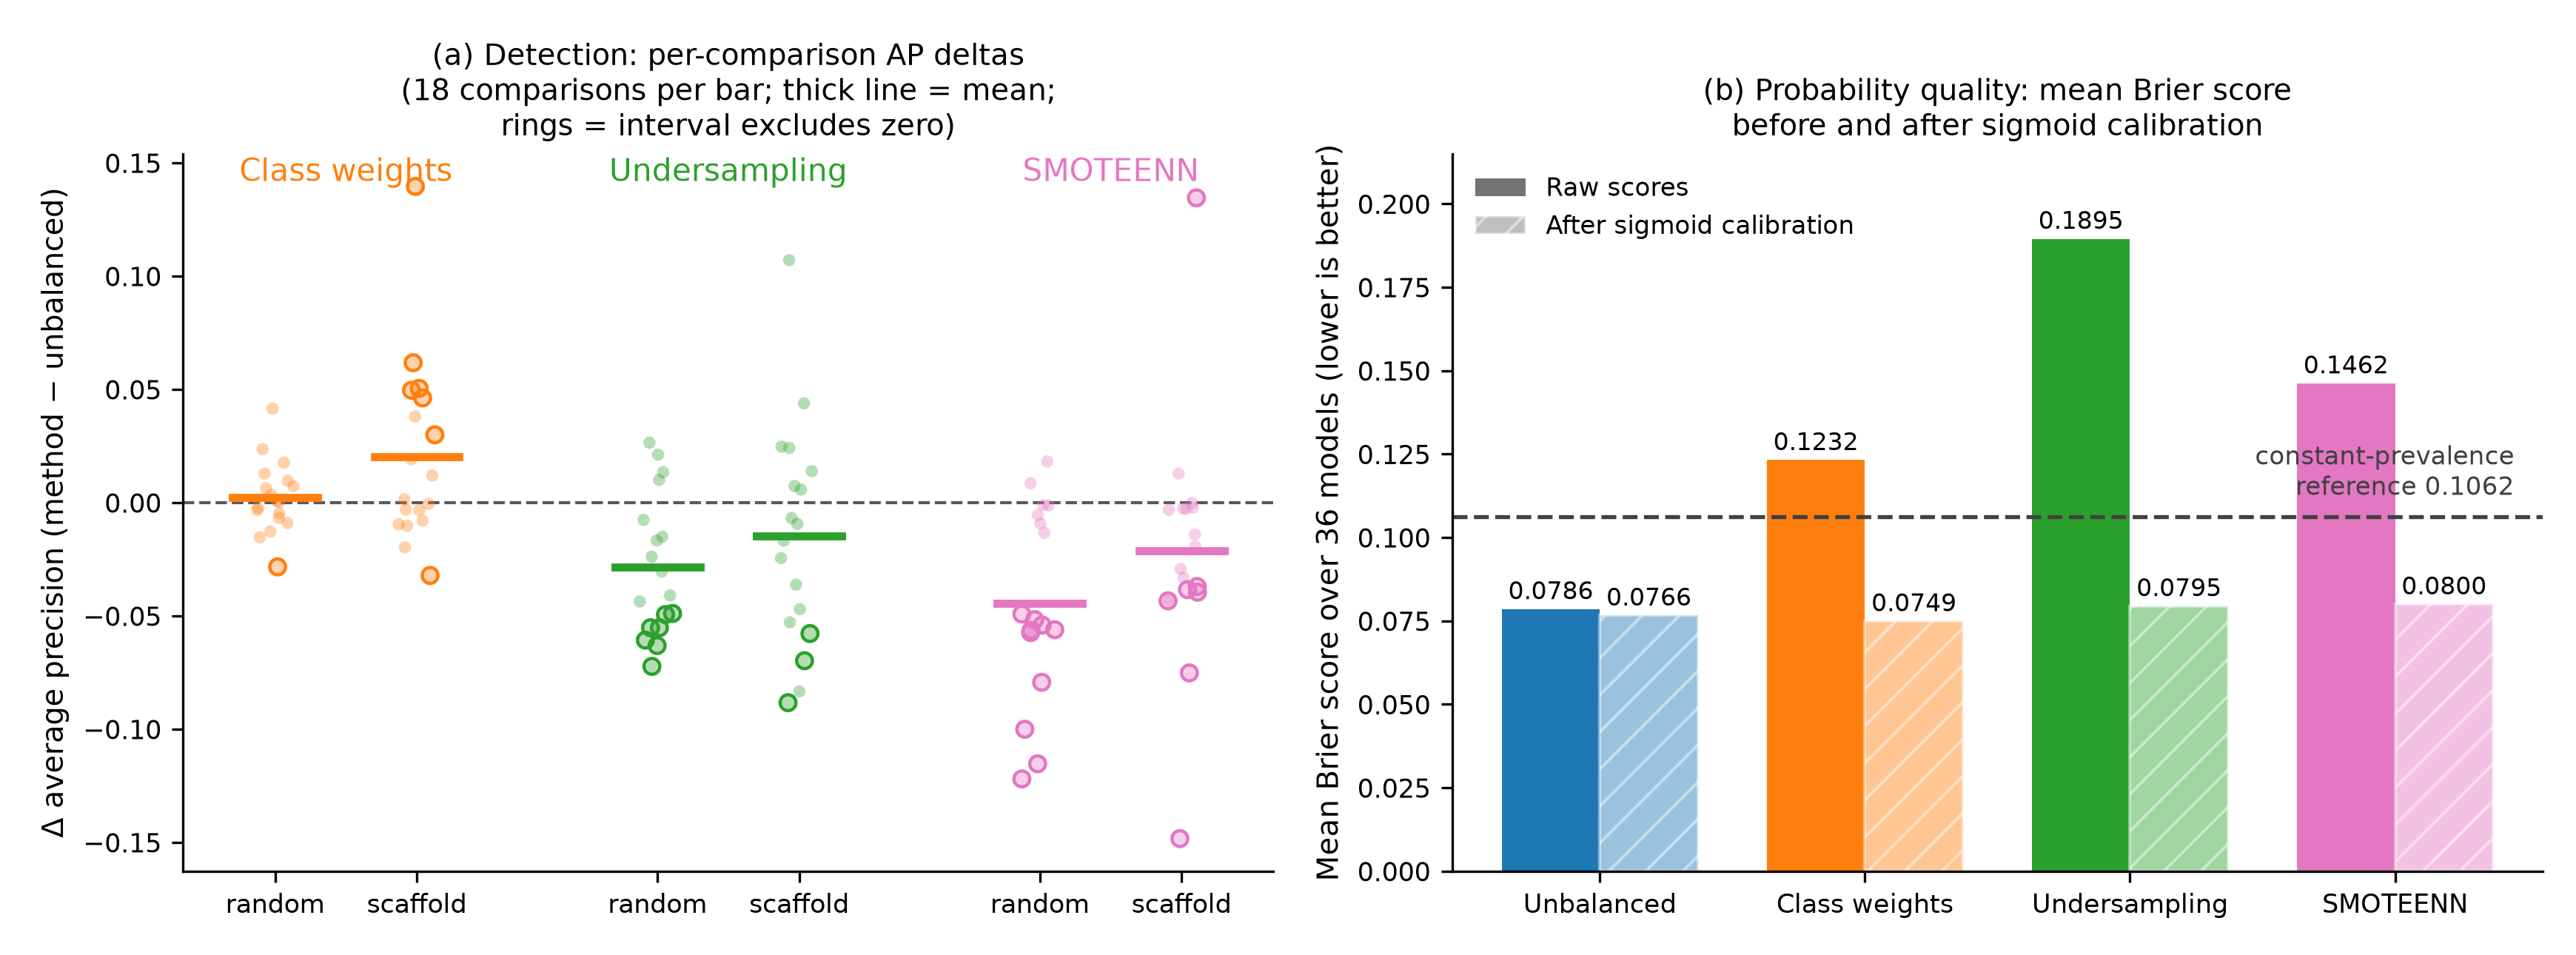
\includegraphics[width=0.92\textwidth]{figures/summary-deltas.png}
\caption{\textbf{(a)} All 108 paired average-precision deltas against the unbalanced baseline,
grouped by balancing method and split kind (18 comparisons per column: 3 assays $\times$ 2
classifiers $\times$ 3 seeds). Thick lines are column means; ringed points mark comparisons whose
95\% percentile bootstrap interval excludes zero. Class weighting is the only method whose mean is
above zero in either split kind. \textbf{(b)} Mean Brier score across the 36 models of each method,
before and after sigmoid calibration, against the constant-prevalence reference (dashed). All three
balancing methods produce raw probabilities worse than the constant reference on average; all four
land well below it after calibration. Generated for this report into \texttt{docs/figures/}.}
\label{fig:summary}
\end{figure}

\subsection{Where the gains are, and how large they are}

\begin{table}[!htbp]
\centering
\small
\caption{Average-precision deltas against the unbalanced baseline, by method, classifier and split
kind (9 comparisons each: 3 assays $\times$ 3 seeds). Positive is favourable.}
\label{tab:apcell}
\begin{tabular}{@{}lllrrrr@{}}
\toprule
Balancing & Classifier & Split & Comparisons & Mean \dd{} AP & Int.\ fav. & Int.\ unfav. \\
\midrule
weights & forest   & random   & 9 & $+0.0040$ & 0 & 1 \\
weights & forest   & scaffold & 9 & $\mathbf{+0.0253}$ & \textbf{4} & \textbf{0} \\
weights & logistic & random   & 9 & $+0.0006$ & 0 & 0 \\
weights & logistic & scaffold & 9 & $+0.0149$ & 2 & 1 \\
\midrule
undersample & forest   & random   & 9 & $-0.0237$ & 0 & 2 \\
undersample & forest   & scaffold & 9 & $+0.0077$ & 0 & 0 \\
undersample & logistic & random   & 9 & $-0.0332$ & 0 & 5 \\
undersample & logistic & scaffold & 9 & $-0.0372$ & 0 & 3 \\
\midrule
SMOTEENN & forest   & random   & 9 & $-0.0482$ & 0 & 4 \\
SMOTEENN & forest   & scaffold & 9 & $-0.0152$ & 0 & 1 \\
SMOTEENN & logistic & random   & 9 & $-0.0409$ & 0 & 6 \\
SMOTEENN & logistic & scaffold & 9 & $-0.0275$ & 1 & 5 \\
\bottomrule
\end{tabular}
\end{table}

\textbf{What gains exist are concentrated in one cell: class weighting with the random forest on the
scaffold split.} In those nine comparisons the delta is favourable in sign seven times, four
intervals exclude zero favourably and none unfavourably, and the mean delta is $+0.0253$. The four
are NR-AhR seeds 42 ($+0.050$ $[+0.006,+0.094]$) and 2026 ($+0.062$ $[+0.013,+0.113]$), and SR-MMP
seeds 42 ($+0.046$ $[+0.001,+0.085]$) and 2026 ($+0.050$ $[+0.022,+0.075]$); the corresponding
seed-mean gains are NR-AhR $0.469\to0.510$ and SR-MMP $0.477\to0.516$. On NR-AR --- the smallest and
most imbalanced assay --- the same combination shows no gain at all ($0.497\to0.493$, no interval
excluding zero).

Two counter-observations keep this from being read as more than it is. The one unfavourable
class-weighting interval on the scaffold split is NR-AhR / logistic / seed 42
($-0.032$ $[-0.056,-0.001]$). And the largest single favourable delta anywhere in the study ---
NR-AR / scaffold / logistic / seed 2026, $+0.140$ $[+0.034,+0.213]$ --- comes from the group with by
far the widest seed-to-seed spread (unbalanced $0.394 \pm 0.121$, class-weighted $0.447 \pm 0.190$);
the same comparison is $-0.020$ on seed 17 and $+0.038$ on seed 42. \emph{That instability, not the
point estimate, is the reportable finding there.}

Figure~\ref{fig:pr} sets the best case beside a representative bad case: the NR-AhR scaffold group
where class weighting helps, and the SR-MMP random group where SMOTEENN and undersampling both cost
precision across the whole useful recall range.

\begin{figure}[!htbp]
\centering
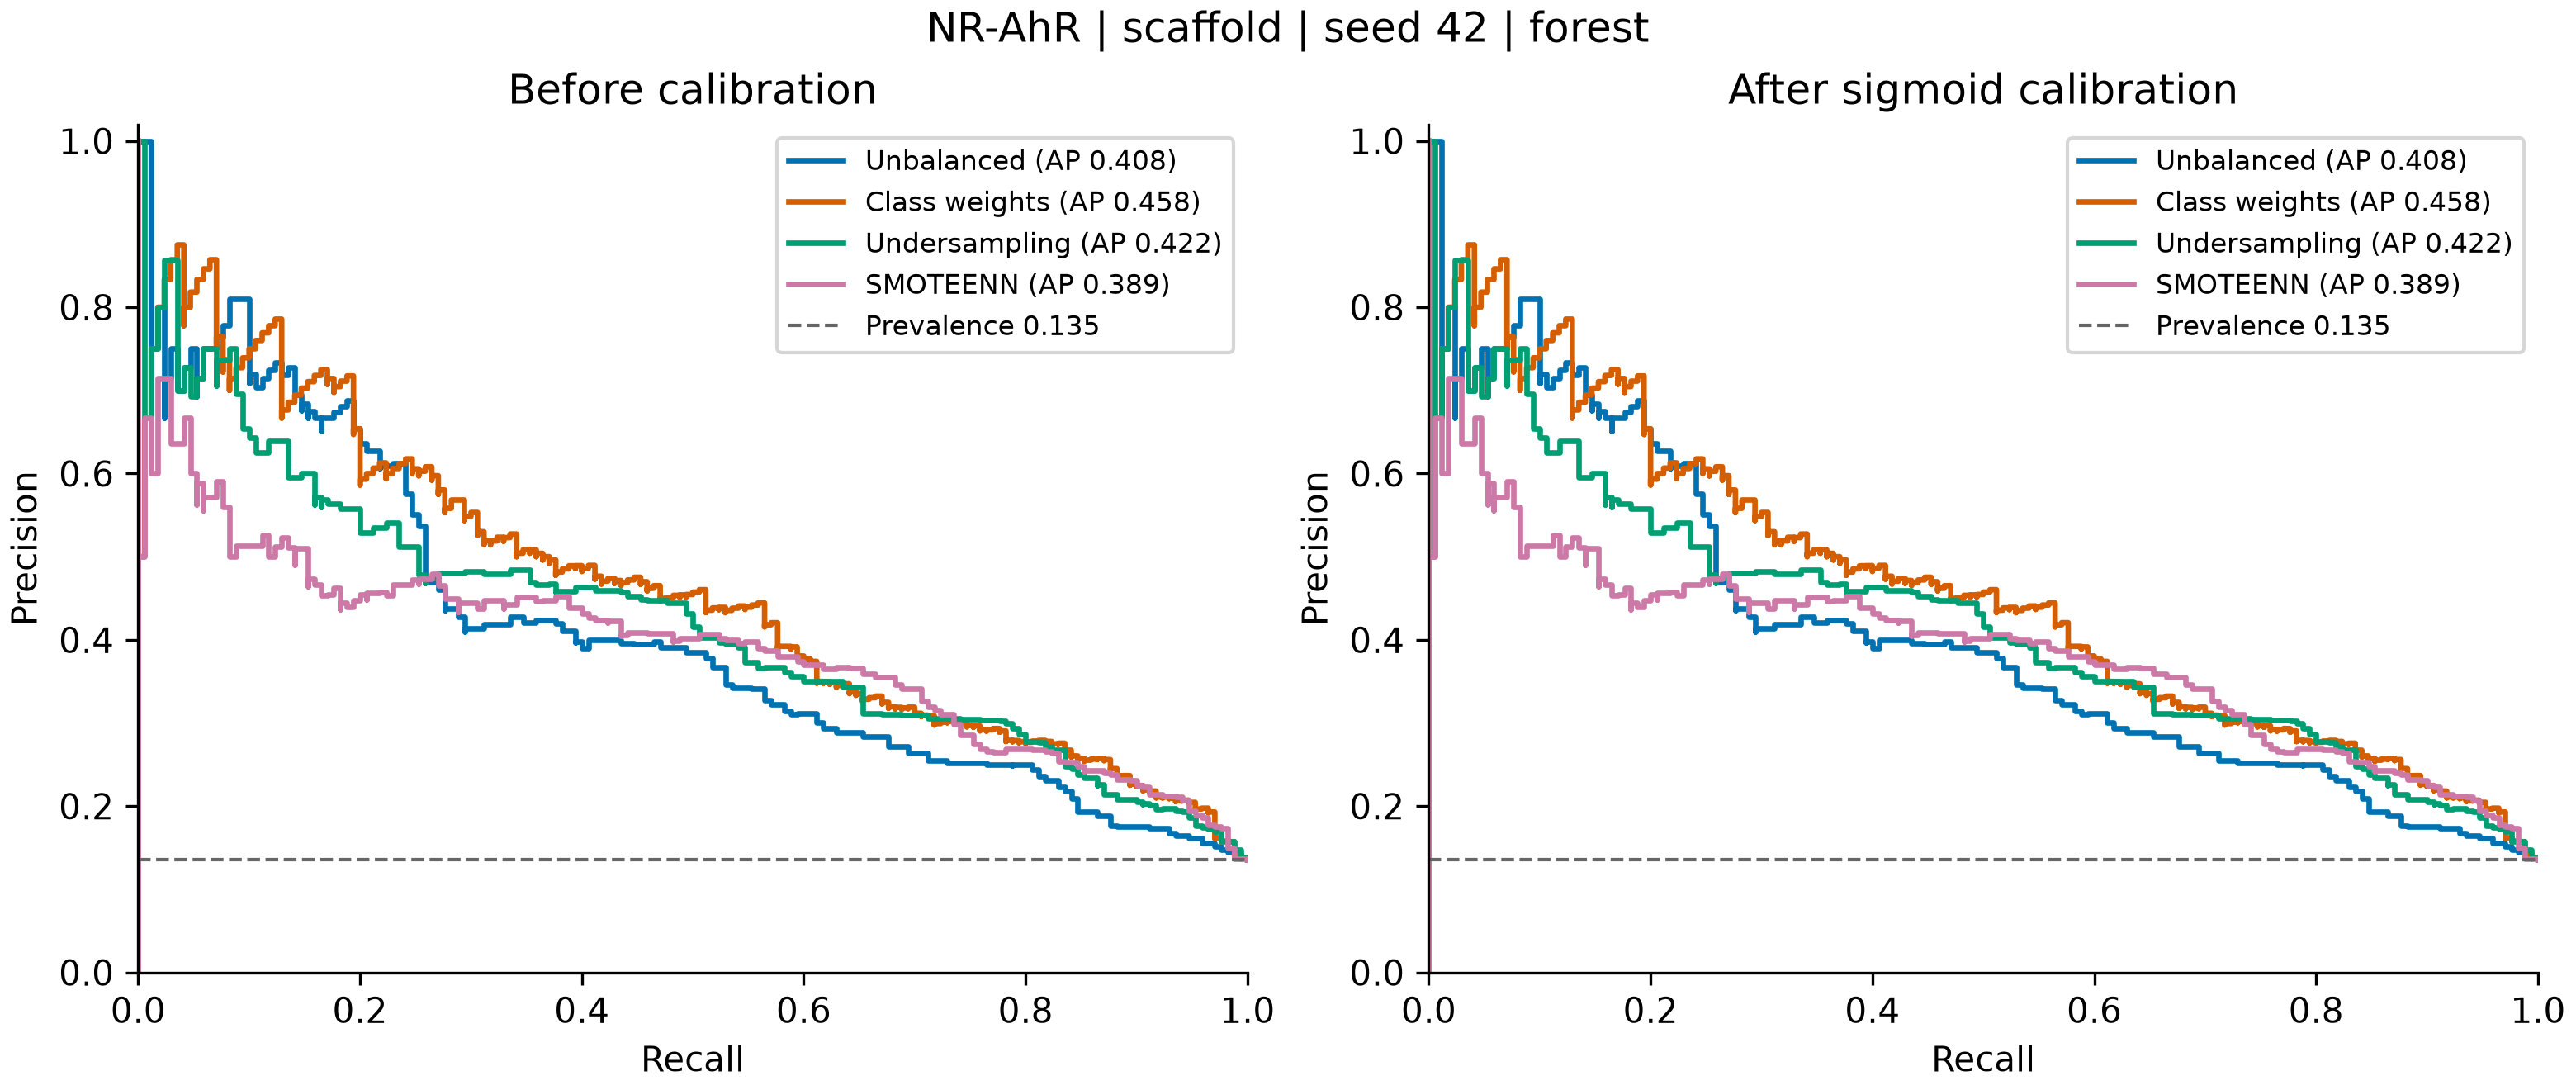
\includegraphics[width=0.76\textwidth]{figures/pr-nrahr-scaffold-42-forest.png}\\[2pt]
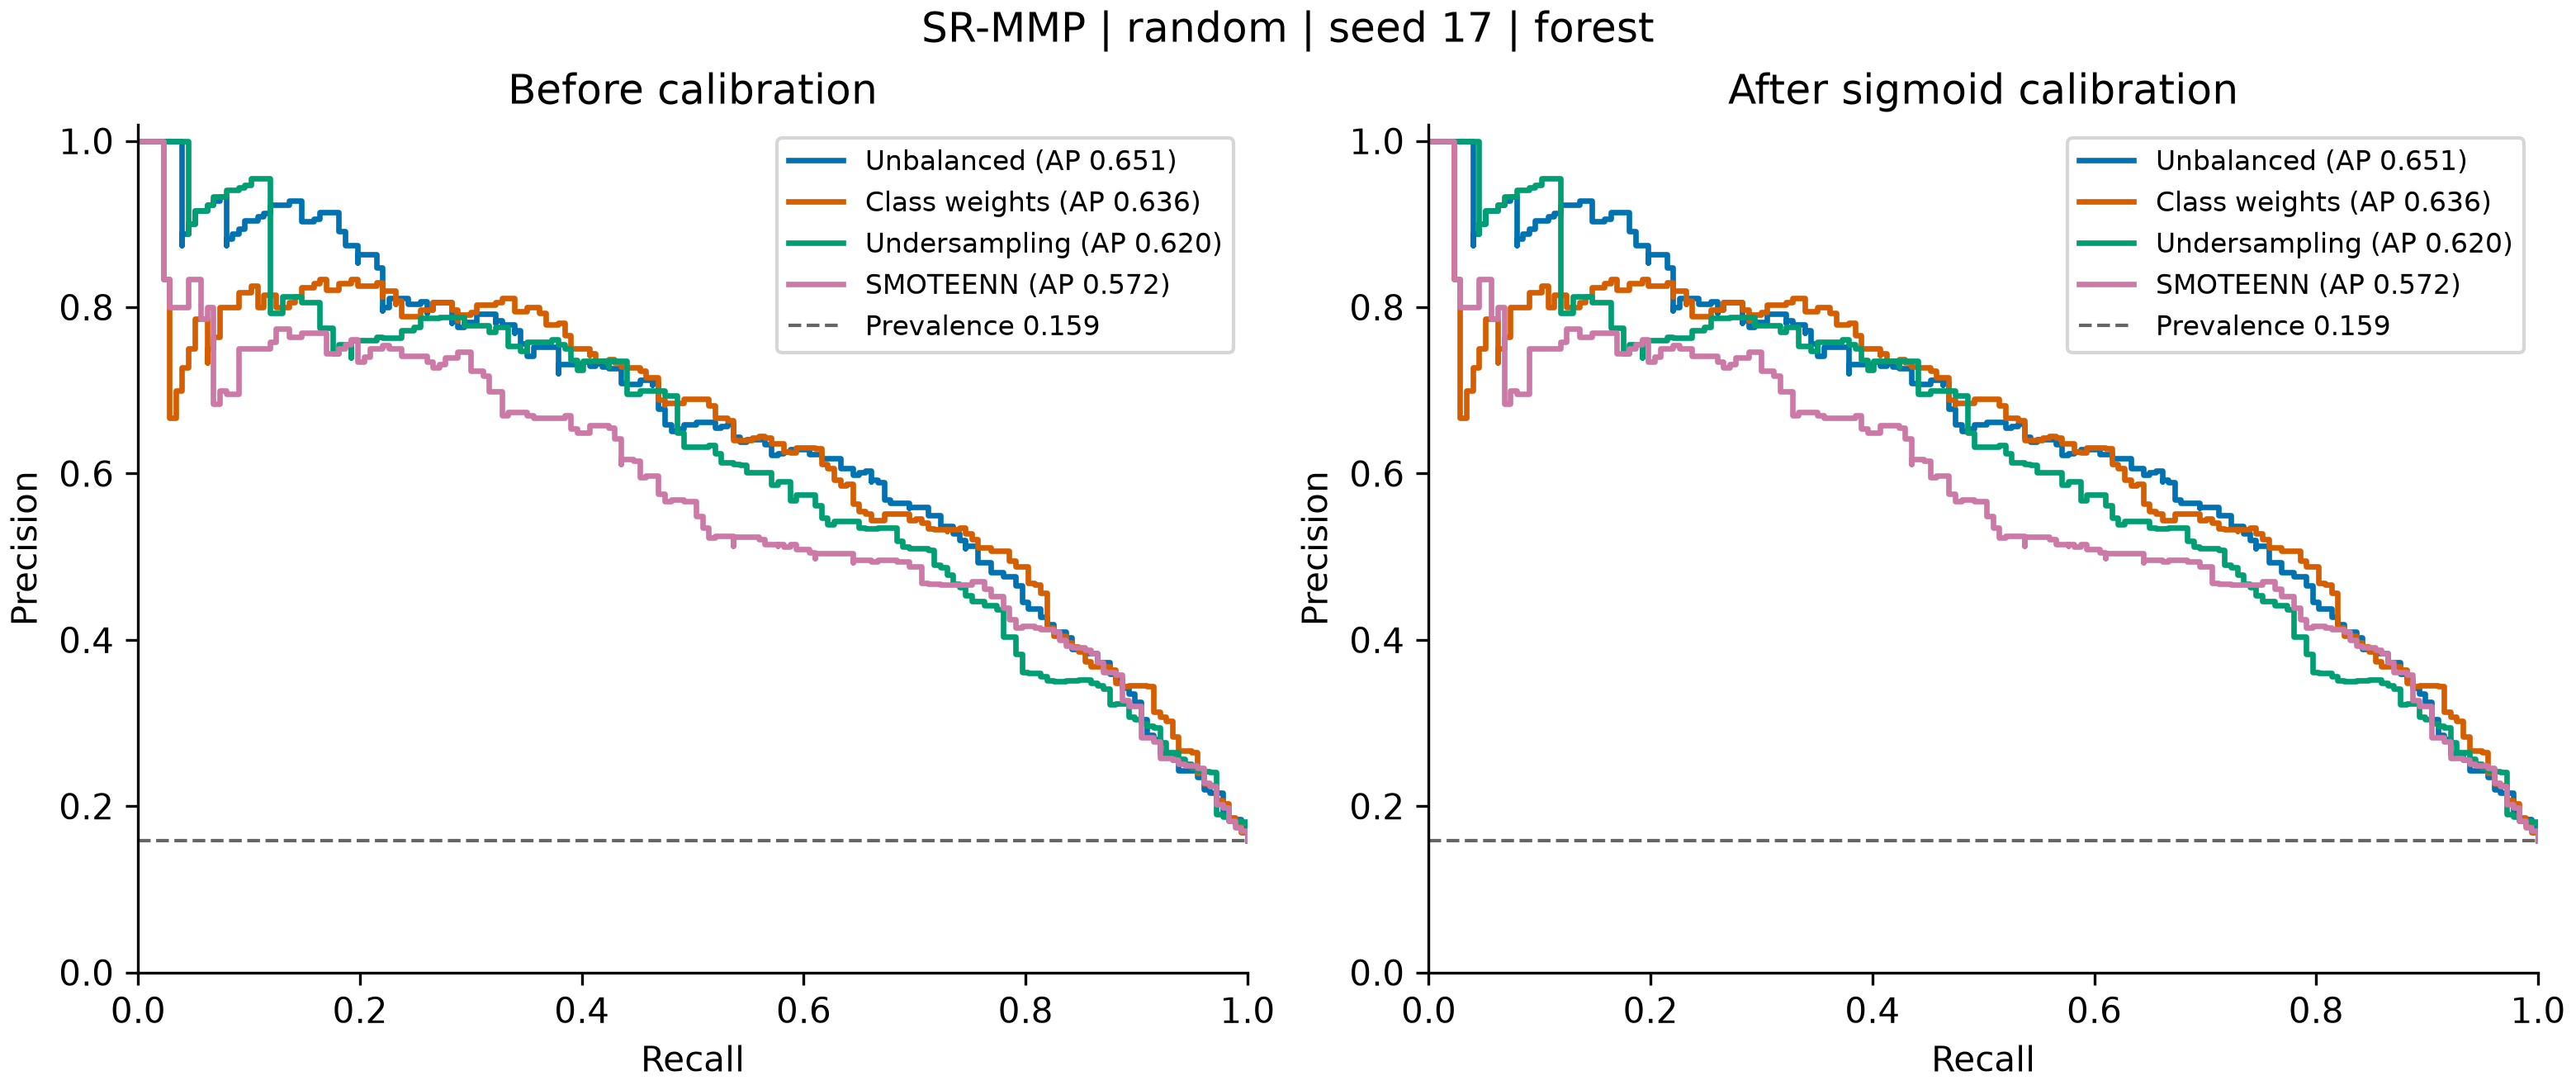
\includegraphics[width=0.76\textwidth]{figures/pr-srmmp-random-17-forest.png}
\caption{Committed precision--recall curves for all four balancing methods, before (left panel) and
after (right panel) sigmoid calibration. \textbf{Top:} NR-AhR, scaffold, seed 42, forest --- the
clearest class-weighting gain (orange above blue through most of the mid-recall range a budget uses;
$0.408 \to 0.458$, interval $[+0.006,+0.094]$). \textbf{Bottom:} the counter-example, SR-MMP,
random, seed 17, forest, where SMOTEENN (pink) loses precision across the whole useful recall range
($0.651 \to 0.572$, $[-0.134,-0.021]$) and undersampling (green, 0.620) also falls below the
baseline. In both plots the two panels are \emph{identical in shape}: a monotone calibration map
cannot move a precision--recall curve, and the legend average precisions agree to the last digit
(Section~\ref{sec:ranking}). Sources:
\texttt{outputs/full/evaluation/NR-AhR/scaffold/42/forest/precision\_recall.png} and
\texttt{.../SR-MMP/random/17/forest/precision\_recall.png}.}
\label{fig:pr}
\end{figure}

\subsection{Why the methods behave the way they do (RQ4)}

Table~\ref{tab:resample} explains the pattern without appeal to anything beyond the data.
\textbf{Undersampling throws away the evidence}: on NR-AR / scaffold / seed 17 it discards 3{,}898 of
4{,}036 inactive compounds --- 96.6\% of the majority class --- and fits on 276 compounds instead of
4{,}174. In a 2{,}048-dimensional binary space those discarded negatives are the only thing defining
where the inactive region is. Cross-validation noticed: undersampling is the only method that
frequently selected a depth-limited forest (Table~\ref{tab:hyper}), the standard response to a much
smaller sample. The loss is worst where there was least imbalance to correct, because there the
method destroys the most data for the least benefit.
\textbf{SMOTEENN manufactures examples that are not molecules}: it introduces 59{,}492--131{,}992
fractional cells into a matrix whose entries are substructure presence indicators, and a model that
learns a boundary in that interpolated space is learning about a region of feature space the test
distribution never visits; its ENN step then deletes real majority examples as well. It is the worst
method here on average precision ($-0.0329$) and the only one with a double-digit count of
unfavourable intervals on that metric (16).
\textbf{Class weighting changes the objective, not the data}: it keeps every compound and every real
feature value and only alters how much a minority error costs. That is why it has no detection cost,
and why its benefit appears where the imbalance is both substantial and informative --- on the
scaffold split with the forest.

\subsection{Calibration cannot change ranking here, and it did not}
\label{sec:ranking}

This result determines what calibration may be credited with, so it is stated before any calibration
effect is reported. The fitted sigmoid is constrained to a nonnegative slope
(Section~\ref{sec:calibimpl}); a monotone non-decreasing map cannot reorder compounds, so it cannot
change any metric that depends only on the ranking. This holds exactly in the stored results: across
all 144 models the maximum absolute difference between raw and sigmoid states is \textbf{exactly 0.0}
for average precision and \textbf{exactly 0.0} for ROC AUC, and the paired bootstrap deltas for
average precision, ROC AUC, precision@10\% and recall@10\% are identical to 0.0 between the two
states. The audit additionally confirmed zero strict rank reversals over all test pairs in all 144
models, with fitted slopes in $[0.510, 1.887]$ and no zero-slope or constant-mapping case.

\begin{quote}
\textbf{Calibration is therefore never presented in this report as improving average precision, ROC
AUC, or any other ranking measure. Its effects belong entirely to Brier score, log loss and the
reliability curves.}
\end{quote}

One related detail. Two of the 144 models --- \texttt{NR-AhR/scaffold/42/forest/none} and
\texttt{SR-MMP/scaffold/17/forest/none} --- record \texttt{rank\_order\_identical: false}. This is
\emph{not} a rank reversal: the audit established that in each case the sigmoid maps two or three
compounds whose raw forest probabilities differ by 1--2 units in the last place of float64 onto a
single float64 value, and that every such collapsed group consists entirely of negatives. Average
precision and ROC AUC are mathematically unchanged; the flag is a strict permutation-equality test
sensitive to float64 tie structure carrying no ranking information.

\subsection{Probability quality: what balancing costs and what calibration repairs}
\label{sec:prob}

\begin{table}[!htbp]
\centering
\small
\caption{Probability quality pooled over the 36 models of each balancing method. \textbf{Lower is
better} for both losses. The last two columns count how many of each method's 36 models have a Brier
score \emph{worse} than the constant-prevalence reference, before and after calibration. The
reference depends only on the partition and is shown once.}
\label{tab:prob}
\begin{tabular}{@{}lrrrrcc@{}}
\toprule
 & \multicolumn{2}{c}{Brier score} & \multicolumn{2}{c}{Log loss} & \multicolumn{2}{c}{Worse than constant} \\
\cmidrule(lr){2-3}\cmidrule(lr){4-5}\cmidrule(lr){6-7}
Balancing & raw & sigmoid & raw & sigmoid & raw & sigmoid \\
\midrule
none (baseline) & 0.0786 & 0.0766 & 0.2810 & 0.2656 & \textbf{0 / 36} & 0 / 36 \\
weights         & 0.1232 & 0.0749 & 0.4010 & 0.2592 & 22 / 36 & 0 / 36 \\
undersample     & 0.1895 & 0.0795 & 0.5728 & 0.2715 & \textbf{36 / 36} & 0 / 36 \\
SMOTEENN        & 0.1462 & 0.0800 & 0.4748 & 0.2733 & 26 / 36 & 0 / 36 \\
\midrule
\textit{constant reference} & \multicolumn{2}{c}{\textit{0.1062}} & \multicolumn{2}{c}{\textit{0.3644}} & --- & --- \\
\bottomrule
\end{tabular}
\end{table}

The answer to RQ2 is blunt. \textbf{In the raw state, 84 of the 144 models produce probabilities
strictly worse, by Brier score, than simply predicting the training prevalence for every compound ---
and all 84 are balanced models.} Every one of the 36 undersampling models falls into this category,
along with 26 of 36 SMOTEENN models and 22 of 36 class-weighting models; \textbf{none of the 36
unbalanced models does}. After sigmoid calibration, \textbf{144 of 144} beat the constant reference.
Mean raw Brier for undersampling, 0.1895, is 2.4 times the unbalanced baseline's 0.0786 and well
above the constant reference's 0.1062; after calibration it is 0.0795, indistinguishable from the
calibrated baseline's 0.0766.

The collapse is equally stark per comparison. Over all 108 Brier comparisons against the baseline,
the largest raw delta is $+0.2495$ and the mean absolute delta 0.0745; in the sigmoid state these
become 0.0221 and 0.0038. For log loss the figures are $+0.8263$ and 0.2061 raw, against 0.0607 and
0.0114 after calibration. Calibration on a separate, uncontaminated partition removes most --- not
all --- of the probability distortion that balancing introduces.

\begin{table}[!htbp]
\centering
\small
\begin{minipage}[t]{0.47\textwidth}
\centering
\caption{Mean predicted probability, pooled over the 36 test partitions of each method, against a
mean test prevalence of 0.1227.}
\label{tab:meanp}
\footnotesize
\begin{tabular}{@{}lrr@{}}
\toprule
Balancing & Raw & After sigmoid \\
\midrule
none (baseline) & 0.1151 & 0.1266 \\
weights         & 0.3028 & 0.1267 \\
undersample     & 0.4222 & 0.1268 \\
SMOTEENN        & 0.3193 & 0.1271 \\
\midrule
\textit{true prevalence} & \multicolumn{2}{c}{\textit{0.1227}} \\
\bottomrule
\end{tabular}
\end{minipage}\hfill
\begin{minipage}[t]{0.50\textwidth}
\centering
\caption{Reliability, averaged over the 12 groups of each method. ``Gap'' is the count-weighted mean
$|$predicted $-$ observed$|$; ``bias'' is the same without absolute value.}
\label{tab:reliab}
\footnotesize
\begin{tabular}{@{}lrrrr@{}}
\toprule
 & \multicolumn{2}{c}{Weighted gap} & \multicolumn{2}{c}{Signed bias} \\
\cmidrule(lr){2-3}\cmidrule(lr){4-5}
Balancing & raw & sigmoid & raw & sigmoid \\
\midrule
none        & 0.0297 & 0.0181 & $-0.0076$ & $+0.0039$ \\
weights     & 0.1815 & 0.0178 & $+0.1801$ & $+0.0040$ \\
undersample & 0.3002 & 0.0217 & $+0.2995$ & $+0.0040$ \\
SMOTEENN    & 0.1989 & 0.0192 & $+0.1966$ & $+0.0044$ \\
\bottomrule
\end{tabular}
\end{minipage}
\end{table}

\textbf{The mechanism: raw balanced models are over-confident toward the positive class.} In the raw
state, balanced models predict a far higher average probability than the data support ---
undersampling's mean prediction of 0.4222 is \textbf{3.4 times} the true mean test prevalence of
0.1227. The signed reliability bias is positive and large for all three balancing methods ($+0.18$ to
$+0.30$), meaning the reliability curve sits well below the diagonal: a bin whose compounds are
assigned around 0.5 contains far fewer than half actives. The unbalanced model is nearly unbiased in
the raw state ($-0.0076$).

A single partition makes this concrete. On NR-AR / scaffold / seed 17 / forest, where the true test
prevalence is 0.0446, mean predicted probabilities are 0.0394 (unbalanced), 0.0924 (weights), 0.1098
(SMOTEENN) and \textbf{0.4122 (undersampling --- 9.2 times too high)}. After sigmoid calibration all
four land between 0.0509 and 0.0560, within about one percentage point of the truth. This is exactly
what Table~\ref{tab:resample} predicts: a model trained on a 1:1 sample has learned a 50\% base rate,
and nothing in its training told it the world is 4.5\% actives.

Sigmoid calibration moves every group onto the diagonal. The weighted gap falls for \textbf{48 of 48}
groups, the post-calibration gap is between 0.0042 and 0.0311 everywhere, and signed bias stays
within $\pm0.018$. The large method-to-method differences in the raw state (0.0297 for \texttt{none}
against 0.3002 for undersampling) essentially disappear afterwards (0.0181 against 0.0217).
Figure~\ref{fig:reliability} shows this directly. One further structural observation: \textbf{the
residual post-calibration gap is larger on scaffold splits than on random splits} --- in all 24
matched assay $\times$ classifier $\times$ method cells, mean weighted gap 0.0235 against 0.0149 ---
consistent with the map being fitted on a scaffold calibration partition whose prevalence differs
from the scaffold test partition's (Table~\ref{tab:partitions}), so the fitted sigmoid is slightly
mismatched to the test distribution.

\begin{figure}[!htbp]
\centering
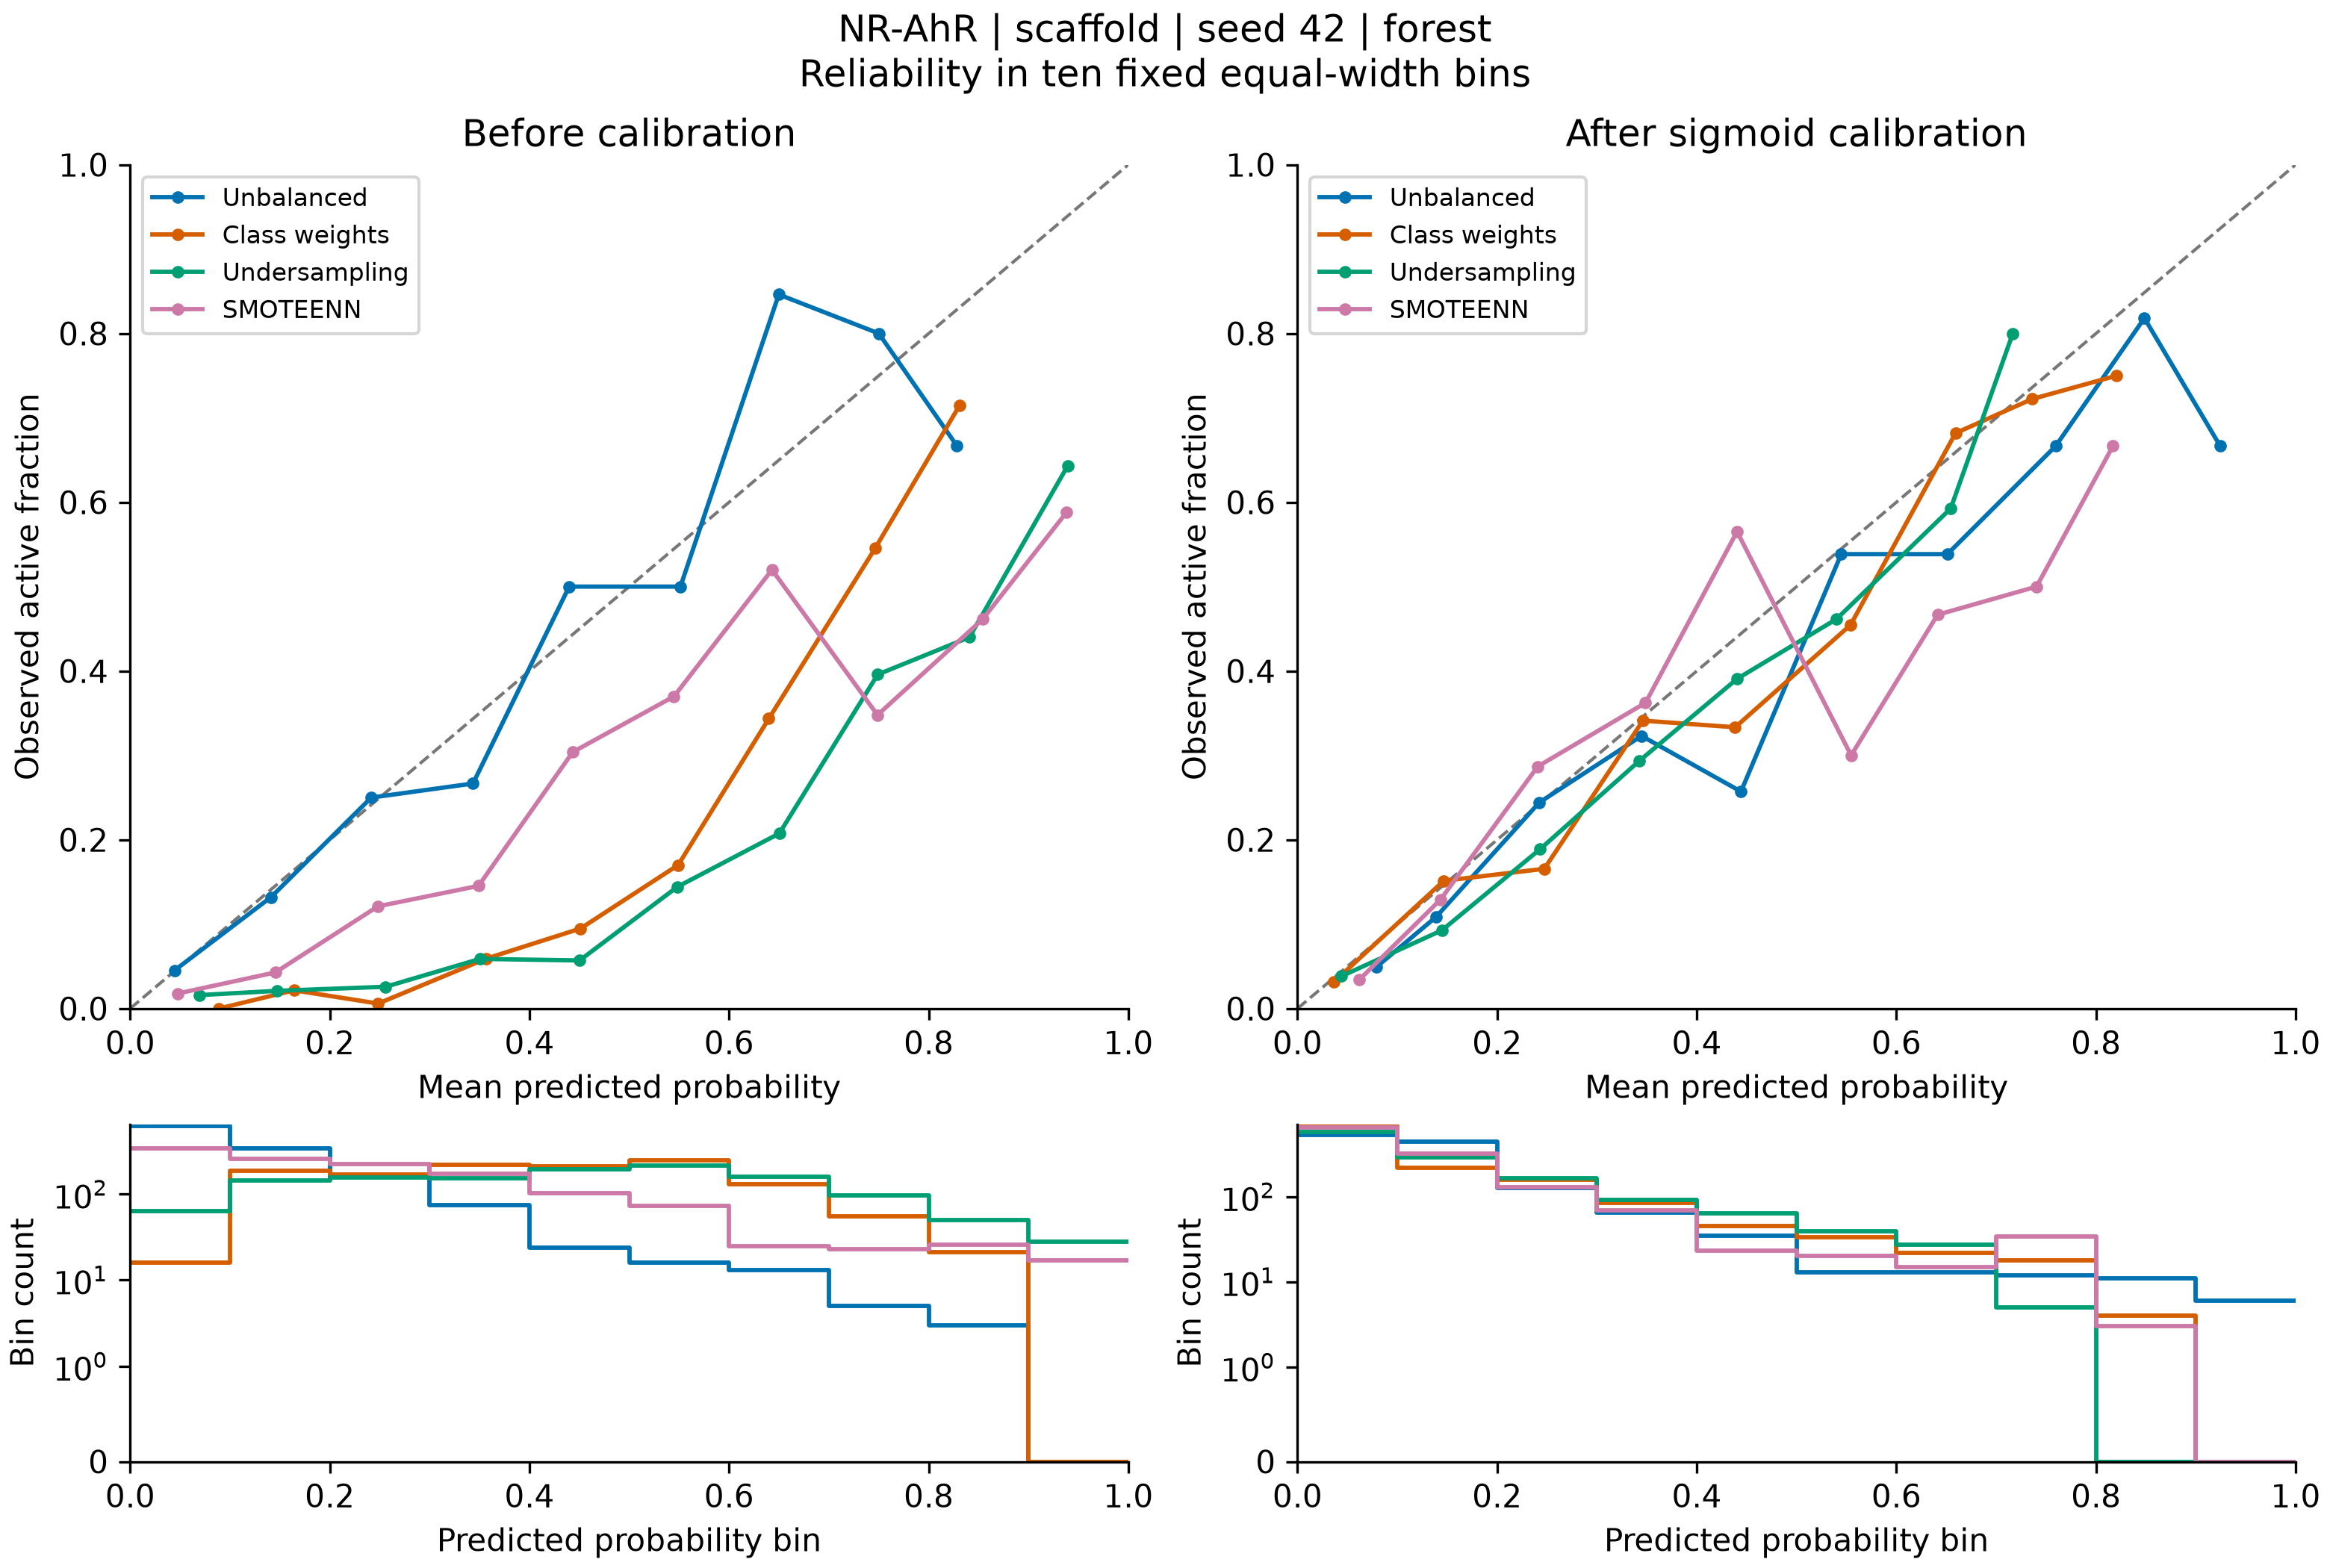
\includegraphics[width=0.64\textwidth]{figures/rel-nrahr-scaffold-42-forest.png}
\caption{Reliability diagrams with bin counts: NR-AhR, scaffold split, seed 42, random forest. Top
left, the raw state --- the unbalanced model (blue) tracks the diagonal while the three balanced
models sit far \emph{below} it; for undersampling (green) the bin predicted near 0.55 contains about
14\% actives. Top right, after calibration all four curves collapse onto the diagonal. Bottom row,
bin counts on a log scale, because a reliability point with four compounds behind it should not be
read like one with four hundred. The compound \emph{ordering} is identical across the two columns.
Source: \texttt{outputs/full/evaluation/NR-AhR/scaffold/42/forest/reliability.png}.}
\label{fig:reliability}
\end{figure}

\begin{table}[!htbp]
\centering
\small
\caption{All models where the sigmoid state is worse than the raw state on Brier score or log loss.
\textbf{Every one is an unbalanced (\texttt{none}) model}; no balanced model appears.}
\label{tab:calworse}
\begin{tabular}{@{}llllrrrrl@{}}
\toprule
Assay & Split & Seed & Classifier & Brier raw & Brier sig. & Log loss raw & Log loss sig. & Worse on \\
\midrule
NR-AR  & random   & 17   & logistic & 0.02690 & 0.02749 & 0.13550 & 0.12513 & Brier \\
NR-AR  & random   & 2026 & logistic & 0.02704 & 0.02705 & 0.12955 & 0.12914 & Brier \\
NR-AR  & scaffold & 42   & logistic & 0.04110 & 0.04124 & 0.17812 & 0.17523 & Brier \\
NR-AR  & scaffold & 2026 & logistic & 0.05097 & 0.05827 & 0.19619 & 0.21499 & \textbf{both} \\
NR-AhR & scaffold & 17   & logistic & 0.10671 & 0.10677 & 0.35413 & 0.35275 & Brier \\
NR-AhR & scaffold & 42   & forest   & 0.09904 & 0.10032 & 0.33516 & 0.34083 & \textbf{both} \\
NR-AhR & scaffold & 42   & logistic & 0.09278 & 0.09281 & 0.31378 & 0.31314 & Brier \\
NR-AhR & scaffold & 2026 & forest   & 0.11404 & 0.11244 & 0.37090 & 0.37122 & log loss \\
\bottomrule
\end{tabular}
\end{table}

\textbf{Cases where calibration made things worse.} The proposal committed to reporting these, and
they exist (Table~\ref{tab:calworse}). 8 of 144 models are worse after calibration on at least one
measure --- 7 on Brier, 3 on log loss, 2 on both --- and \textbf{all of them are unbalanced models}:
the models already close to well calibrated in the raw state, which therefore had nothing to gain and
a little to lose from fitting a two-parameter map on a finite calibration partition. The largest
single degradation is NR-AR / scaffold / seed 2026 / logistic, where Brier rises from 0.05097 to
0.05827 and log loss from 0.19619 to 0.21499 --- the same high-variance group flagged in
Section~\ref{sec:detect}. \textbf{No balanced model was made worse by calibration on either measure.}

\subsection{Scaffold versus random: does any benefit survive the harder split?}
\label{sec:scaffvrand}

\begin{table}[!htbp]
\centering
\small
\caption{Scaffold versus random evaluation, paired within assay, classifier and balancing method (24
cells, raw state). The prevalence-normalised ratio is average precision divided by test prevalence,
which corrects for the higher prevalence of the scaffold test partitions.}
\label{tab:scaffvrand}
\begin{tabular}{@{}lrrrl@{}}
\toprule
Quantity & Random (mean) & Scaffold (mean) & Change & Cells moving that way \\
\midrule
Average precision & 0.5719 & 0.4720 & $-0.0999$ & \textbf{24 / 24 lower} \\
AP $\div$ test prevalence & --- & --- & lower & \textbf{24 / 24 lower} \\
ROC AUC & 0.8290 & 0.7749 & $-0.0541$ & --- \\
Recall @10\% & 0.4899 & 0.3849 & $-0.1051$ & --- \\
Across-seed SD of AP & 0.0379 & 0.0921 & $\times 2.43$ & \textbf{24 / 24 larger} \\
\bottomrule
\end{tabular}
\end{table}

\textbf{The scaffold split is harder, without exception.} Average precision is lower in all 24 cells,
mean change $-0.0999$. Crucially the prevalence-normalised ratio is also lower in all 24, so the drop
is not an artefact of differing test prevalence --- it is in fact \emph{larger} than the raw numbers
suggest, because scaffold test partitions have the higher prevalence and therefore the higher
average-precision floor. Across-seed variability more than doubles. The effect is largest on SR-MMP
(forest, unbalanced: $0.662 \to 0.477$, ratio $4.16 \to 2.31$) and on NR-AR with logistic regression
($0.537 \to 0.394$). This matches the proposal's stated expectation that performance on unfamiliar
scaffolds would be weaker \emph{and} less stable, and it is the most robust single result in the
study.

Does any balancing benefit survive? \textbf{One narrow benefit does, and it is clearer on the
scaffold split than on the random split, but it does not hold across all three assays.}
\emph{Class weighting with the random forest} is essentially neutral on the random split
($+0.0040$) and the strongest result in the study on the scaffold split ($+0.0253$, 4 of 9
favourable intervals, none unfavourable), on NR-AhR and SR-MMP but not NR-AR. \emph{With logistic
regression} it is neutral on random ($+0.0006$) and positive on average on scaffold ($+0.0149$), but
driven almost entirely by the single unstable NR-AR / seed 2026 comparison. \emph{Undersampling and
SMOTEENN} are harmful on average under both split kinds; their scaffold averages are less negative
than their random averages (undersampling $-0.0148$ against $-0.0284$; SMOTEENN $-0.0213$ against
$-0.0445$), but ``less harmful on the harder split'' is not a benefit surviving, and neither
accumulates favourable intervals anywhere near the number of unfavourable ones.

Two cautions attach to the surviving benefit. First, Section~\ref{sec:scaffcaveat}: the scaffold test
set is the remaining scaffold distribution after two giant groups are placed in training, so
``scaffold split'' here does not mean a uniform draw over new scaffolds. Second, those four deltas
span $+0.046$ to $+0.062$ average precision, on two of three assays with three overlapping seeds,
against unadjusted intervals. That is a direction worth following up; it is not an established
effect.

\subsection{Similarity analysis: why the scaffold split is harder}
\label{sec:similarity}

Nearest-neighbour Tanimoto thresholds were fixed before any result was viewed, in four bins. Each
test compound is assigned to the bin containing its maximum Tanimoto similarity to any training
compound, and metrics are recomputed within the bin.

\begin{table}[!htbp]
\centering
\small
\caption{Average precision by nearest-neighbour Tanimoto similarity bin, pooled over all 72 series
per split kind (assay $\times$ seed $\times$ classifier $\times$ balancing method), with mean bin
composition per partition. Raw state.}
\label{tab:simbins}
\begin{tabular}{@{}lrrrrl@{}}
\toprule
 & \multicolumn{2}{c}{Random split} & \multicolumn{2}{c}{Scaffold split} & \\
\cmidrule(lr){2-3}\cmidrule(lr){4-5}
Tanimoto bin & mean AP & mean $n$ / pos. & mean AP & mean $n$ / pos. & \\
\midrule
$[0.0, 0.4)$ & 0.330 & 268 / 26 & 0.348 & 636 / 72 & \\
$[0.4, 0.6)$ & 0.531 & 494 / 51 & 0.548 & 475 / 74 & \\
$[0.6, 0.8)$ & 0.684 & 353 / 39 & 0.622 & 126 / 19 & \\
$[0.8, 1.0]$ & 0.743 & 139 / 13 & \textit{0.498} & \textit{17 / 1} & \textbf{exploratory} \\
\bottomrule
\end{tabular}
\end{table}

\textbf{Performance rises with similarity to the training set, in every single series.} Across all 48
assay $\times$ split $\times$ classifier $\times$ method series, average precision in the $[0.6,0.8)$
bin exceeds that in $[0.0,0.4)$ \textbf{48 out of 48 times}, and the increase is monotone across the
first three bins in 45 of 48; ROC AUC, which does not depend on bin prevalence, shows the same
ordering in 47 of 48. The low-similarity bin is genuinely the hard regime: for NR-AR random splits
the unbalanced forest scores 0.157 average precision in $[0.0,0.4)$ against 0.686 in $[0.6,0.8)$.

\textbf{The scaffold split does not create a different problem; it reweights the same one.} The
scaffold $[0.0,0.4)$ bin holds 579--696 compounds per partition where the random one holds 232--300,
while the scaffold $[0.8,1.0]$ bin collapses to 12--25 compounds, and mean nearest-neighbour
similarity falls from ${\sim}0.56$ to ${\sim}0.42$ (Table~\ref{tab:tanimoto}). The scaffold split is
harder largely because it loads the test set with more unfamiliar compounds.

\textbf{The scaffold top bin must not be over-read.} Average precision in $[0.8,1.0]$ exceeds
$[0.6,0.8)$ in 22 of 24 random-split series but only 8 of 24 scaffold-split series. \textbf{Every
scaffold $[0.8,1.0]$ bin is exploratory in every seed} (12--25 compounds, 0--3 positives), so those
values are dominated by sampling noise; the apparently dramatic NR-AR / scaffold / logistic /
undersampling value of 0.500 in that bin rests on a single positive compound. Relatedly,
\texttt{similarity\_metrics.csv} contains 32 undefined average-precision values and 32 undefined ROC
AUC values. These are \emph{not} missing data and not a computation failure: two bins (NR-AR /
scaffold, seeds 17 and 2026, $[0.8,1.0]$, 12 and 15 compounds) contain \textbf{zero positives}, both
metrics are mathematically undefined for a single-class subset, and each bin contributes 16 rows
(2 classifiers $\times$ 4 methods $\times$ 2 calibration states).

\textbf{Balancing does not change the similarity gradient.} Class weighting with the forest on the
scaffold split does improve average precision in the low-similarity bin for NR-AhR
($0.364 \to 0.423$) and SR-MMP ($0.403 \to 0.422$), consistent with the aggregate result, but no
method flattens the gradient or lifts the $[0.0,0.4)$ bin anywhere near the higher-similarity bins.

\subsection{Comparison with published work}

A like-for-like numerical comparison with [1], [2] or [4] is not available, and claiming one would be
misleading: curation rules, descriptor sets, tuning grids and split procedures all differ, and two of
those references are verified only at the abstract level. What can be compared is direction.

The clearest point of contact is van den Goorbergh et al.~[3], who found that imbalance corrections
distorted predicted risks in logistic regression without improving discrimination. These results are
\textbf{directionally consistent} in a different setting: here too, resampling moved the probabilities
dramatically (mean raw Brier $0.0786 \to 0.1895$ for undersampling, signed reliability bias up to
$+0.2995$) while the ranking gained nothing on average ($-0.0216$ for undersampling, $-0.0329$ for
SMOTEENN). The agreement is notable because [3]'s evidence came from simulations and a clinical case
study with a handful of covariates, whereas this evidence comes from 2{,}048-bit fingerprints and
includes a tree ensemble as well as a linear model --- but it remains suggestive rather than
confirmatory, because the settings differ in almost every respect except the mechanism tested.

The relationship with Idakwo et al.~[1] is more complicated: SMOTEENN was included here
\emph{because} it performed well there, and in this benchmark it was the worst of the three methods
on detection. That is not a contradiction of [1] --- curation, bagging design, descriptors, tuning
and model-selection protocol all differ --- but it is a concrete reason to be cautious about
transferring a balancing recommendation between Tox21 studies without re-testing it.

\subsection{Limitations}

Ordered roughly by how much they constrain the conclusions.

\begin{enumerate}\setlength{\itemsep}{1pt}
\item \textbf{The scaffold test set is not a uniform draw over scaffolds.} The fixed size-based
allocator places \texttt{\_\_EMPTY\_\_} and benzene --- together 41.9--44.7\% of each assay and
69.9--74.6\% of each training partition --- into training every time (Table~\ref{tab:giant}).
``Performance on new scaffolds'' here therefore means performance on the remaining distribution of
smaller, more peripheral scaffold groups. This is a deliberate consequence of a pre-registered,
label-independent rule that never splits a group.

\item \textbf{Three seeds are not independent replication.} The seeds draw overlapping test sets from
the same cleaned assay table, so the \pmx{} values are split and fit variation, not sampling error
over datasets. Scaffold cross-validation folds are additionally distorted by the same giant groups
(deviations up to 7.91 pp from equal thirds; one NR-AR fold with 14 positives and one NR-AhR fold
with 18, both exploratory, for every seed), which makes hyperparameter selection on those assays less
stable than the grid search implies.

\item \textbf{The intervals are conditional and unadjusted.} Every interval conditions on the
already-fitted model and the current test partition, capturing test-set sampling variability only ---
not retraining, not resampling of the split, not generalisation to other assays. Several hundred such
comparisons are made with no multiplicity adjustment. Intervals excluding zero are reported as a
descriptive feature of one test partition and nothing more.

\item \textbf{The two classifiers' intervals within a partition are not independent evidence.} The
bootstrap RNG seed is derived at \texttt{toxbench/postprocess.py:32} as
\texttt{sha256(assay/kind/seed)}, which \textbf{excludes the classifier}. Within a given assay, split
kind and partition seed, the logistic and forest groups therefore draw the \emph{identical} 1{,}000
resample index vectors. The pairing within each classifier is correct and the intervals are valid,
but wherever this report notes that a result appears for both classifiers in the same partition,
those two intervals rest on the same resamples and must not be read as two independent
confirmations. A related naming hazard: the \texttt{seed} column in
\texttt{bootstrap\_differences.csv} holds the \emph{partition} seed, not the bootstrap RNG seed.

\item \textbf{Small positive counts.} NR-AR is the limiting case: 298 positives in 6{,}957 structures,
giving test partitions with 60--96 positives. Several similarity bins fall below the 20-positive
exploratory threshold, and two scaffold $[0.8,1.0]$ bins contain no positives at all. Conclusions
about NR-AR, and about any bin flagged exploratory, carry correspondingly less weight.

\item \textbf{Narrow design space.} One fingerprint, one calibration family, four-entry grids, two
classifiers, three of twelve assays. Results may not transfer to other descriptors, to isotonic or
beta calibration, to larger grids, or to the nine Tox21 assays not studied. The audit also notes that
no two grid entries ever tied on cross-validated mean average precision, so the documented ``ties go
to the first grid entry'' rule rests on reading the code rather than on an observed event.

\item \textbf{Chemistry and label limitations.} Tautomers are not canonicalised, so residual
tautomer-related near-duplicates may remain across partitions. Tanimoto similarity on binary Morgan
fingerprints is a crude proxy for chemical relatedness, and the Bemis--Murcko scaffold is a coarse
grouping --- most visibly in the single \texttt{\_\_EMPTY\_\_} group pooling every acyclic compound.
Tox21 labels themselves carry assay noise this study does not model.

\item \textbf{Literature context is not a validated baseline.} Reference [1] is fully verified and
motivates the inclusion of SMOTEENN, but its curation, descriptors and tuning differ, so its results
are motivation and not a comparable baseline. Reference [3] is fully verified and directionally
consistent with Sections~\ref{sec:detect} and \ref{sec:prob}, but its evidence comes from simulations
and a clinical case study, so the agreement is suggestive rather than confirmatory. \textbf{Reference
[2] is verified only as bibliographic metadata and abstract, and reference [4] only as bibliographic
metadata and publisher abstract; in particular the proposal's specific assertion about [4]'s use of
class weighting for its tree models was not independently verified and is not asserted as confirmed
anywhere in this report.} The full verification record is \texttt{docs/references.md}.

\item \textbf{Scope of the endpoint.} Restating Section 2: these are assay activity predictions, not
determinations of human toxicity.
\end{enumerate}

% ======================================================================
\section{Conclusions and Future Work}
% ======================================================================

\textbf{Were the objectives achieved?} Yes, with the qualifications below. The complete 144-model
factorial design proposed in Phase 1 ran to completion with zero failed configurations, under two
independent audits (37 data checks, 63 modelling checks) that found no correctness defect and no
test-driven selection. Both halves of the research question were answered with paired,
within-partition evidence, and the pre-registered rule that a rank-preserving calibration may never
be credited with a ranking gain was not merely followed but verified.

\textbf{On detection (RQ1).} Only inverse-frequency class weighting avoided systematically
reducing the number of actives found within a fixed 10\% screening budget (mean $\Delta$ average
precision $+0.0112$ over 36 comparisons; 6 favourable intervals against 2 unfavourable; on ROC AUC,
8 favourable and \emph{zero} unfavourable). Random undersampling ($-0.0216$) and SMOTEENN
($-0.0329$) reduced detection more often than they improved it under both split designs.

\textbf{On new scaffolds (RQ3).} The one combination with interval-supported gains was class
weighting with the random forest on the scaffold split: mean $\Delta$ average precision $+0.0253$
across nine comparisons, four intervals excluding zero favourably and none unfavourably, from two of
three assays --- NR-AhR ($0.469 \to 0.510$) and SR-MMP ($0.477 \to 0.516$) --- and absent on NR-AR.
This is a two-of-three-assay, three-overlapping-seed, unadjusted-interval result on a scaffold test
set that excludes the two largest scaffold groups by construction: a direction worth testing further,
not an established effect.

\textbf{On probability quality (RQ2).} Balancing degrades predicted probabilities badly and
consistently: in the raw state 84 of 144 models are worse by Brier score than predicting the training
prevalence for every compound --- including every one of the 36 undersampling models --- and all 84
are balanced. Sigmoid calibration on a separate, uncontaminated partition repairs most of this: all
144 models beat the constant reference afterwards, the weighted reliability gap improves for all 48
groups, and the largest Brier delta between any balanced method and the baseline falls from
$+0.2495$ to 0.0221. It is not costless --- 8 models came out worse on at least one loss, all of them
unbalanced models that were already nearly calibrated --- but it is close to a prerequisite for using
any balanced model's output as a probability.

\textbf{On what calibration does not do.} Calibration did not improve ranking, and could not have.
Average precision and ROC AUC are identical between raw and sigmoid states for all 144 models
($\max|{\rm raw}-{\rm sigmoid}| = 0.0$), because the fitted sigmoid is constrained to a nonnegative
slope and no model's unconstrained fit wanted a negative one. Every gain reported here is a gain in
probability quality, never in which compounds would be selected.

\textbf{On the harder split.} Testing on held-out scaffolds was uniformly harder: average precision
fell in all 24 cells (mean $-0.0999$), the prevalence-normalised ratio fell in all 24, and across-seed
variability rose by a factor of 2.43. The similarity analysis shows why --- performance rises with
nearest-neighbour Tanimoto similarity in all 48 series tested, and the scaffold split shifts test
mass into the lowest-similarity bin.

\subsection{Practical recommendation and lessons learned}

For this benchmark the defensible recommendation is: \textbf{train without resampling; use
inverse-frequency class weights if anything, since they are the only option here that did not cost
detection and the only one with interval-supported gains on the harder split; and calibrate on a
separate partition before treating any output as a probability.} Resampling the training data bought
no reliable detection benefit and cost a great deal of probability quality that calibration then had
to undo.

Four lessons generalise beyond this dataset. \textbf{(1) Detection and calibration are different
questions and must be reported separately} --- reporting only raw Brier scores would have concluded
that balancing is catastrophic; reporting only post-calibration Brier scores would have concluded it
is free; neither is true. \textbf{(2) Verify rank-invariance rather than assuming it} ---
constraining the calibration slope and then \emph{checking} that all 144 models give identical
average precision in both states is what makes the ``calibration never improves ranking'' claim a
result rather than a hope. \textbf{(3) The evaluation design mattered more than the model} --- the
scaffold-versus-random gap ($-0.0999$) is roughly four times the largest balancing effect found
($+0.0253$), so a study that varied only the model and kept a random split would have drawn
confident conclusions about the wrong quantity. \textbf{(4) A split can be label-independent and
still be structured} --- the scaffold allocator never sees a label, yet two giant groups land in
training every time, which narrows what the primary result can claim.

\subsection{Future work}

\begin{itemize}\setlength{\itemsep}{1pt}
\item \textbf{Settle the surviving effect.} Whether the forest-plus-class-weights gain on unfamiliar
scaffolds is real cannot be decided by three assays and three overlapping seeds. The natural next
step is all twelve Tox21 assays with more seeds and, critically, an \emph{independent} compound
collection with compatible assays and no overlapping structures --- the research extension sketched
in the proposal.
\item \textbf{Fix the scaffold-allocation bias.} Capping giant group sizes, splitting the
\texttt{\_\_EMPTY\_\_} group by a secondary criterion, or using a balanced allocator with an explicit
test-coverage target would make ``performance on new scaffolds'' mean what the phrase implies. Any
such change must remain label-independent and be fixed before results are seen.
\item \textbf{Widen the calibration axis.} Only a two-parameter sigmoid was tested. Isotonic
regression, beta calibration, and calibration fitted on a scaffold-matched partition would test
whether the residual scaffold-split calibration gap (0.0235 against 0.0149) is a property of the
sigmoid family or of the prevalence mismatch.
\item \textbf{Widen the representation axis.} One fingerprint was used throughout, deliberately, so
that differences could be attributed to balancing. Counted fingerprints, different radii,
physicochemical descriptors and learned molecular representations would test the mechanism proposed
in Section 7.3 --- that SMOTE's interpolations are meaningless in a binary substructure space ---
since it predicts SMOTEENN should hurt less in a continuous descriptor space.
\item \textbf{Make the uncertainty honest about retraining.} The current intervals condition on
fitted models. Repeating the fit across bootstrap resamples of the \emph{training} partition, or
across many more split seeds, would capture variation that currently appears only as a three-seed
standard deviation --- and, separately, the bootstrap RNG seed should include the classifier so that
cross-classifier agreement becomes genuine independent evidence.
\end{itemize}

% ======================================================================
\section{References}
% ======================================================================

Scholarly sources are numbered as in the Phase 1 proposal. Verification status reflects
\texttt{docs/references.md}, checked 25 November 2026.

\begin{enumerate}\setlength{\itemsep}{2pt}
\item G. Idakwo, S. Thangapandian, J. Luttrell, Y. Li, N. Wang, Z. Zhou, H. Hong, B. Yang, C. Zhang,
and P. Gong (2020). \emph{Structure-activity relationship-based chemical classification of highly
imbalanced Tox21 datasets}. Journal of Cheminformatics, 12, 66.
DOI: \href{https://doi.org/10.1186/s13321-020-00468-x}{10.1186/s13321-020-00468-x}.
\emph{Verified: full article accessible.}

\item F. Santiago-Gonzalez, J. L. Martinez-Rodriguez, C. Garc\'ia-Perez, A. Juarez-Saldivar, and
H. E. Camacho-Cruz (2025). \emph{Hybrid Class Balancing Approach for Chemical Compound Toxicity
Prediction}. Current Computer-Aided Drug Design, 21(8), 1093--1107. DOI:
\href{https://doi.org/10.2174/0115734099315538240909101737}{10.2174/0115734099315538240909101737}.
\emph{Verified: bibliographic metadata and publisher abstract only; full text paywalled and not
purchased; detailed methods not independently verified.}

\item R. van den Goorbergh, M. van Smeden, D. Timmerman, and B. Van Calster (2022). \emph{The harm of
class imbalance corrections for risk prediction models: illustration and simulation using logistic
regression}. Journal of the American Medical Informatics Association, 29(9), 1525--1534.
DOI: \href{https://doi.org/10.1093/jamia/ocac093}{10.1093/jamia/ocac093}.
\emph{Verified: full article accessible.}

\item Kartic, Y. Seo, S. Yi, and T.-S. Park (2026). \emph{ToxBench: a leakage-audited multi-task
benchmark for predictive toxicology with calibration, uncertainty, and applicability domain
analysis}. BMC Bioinformatics, published 5 September 2026.
DOI: \href{https://doi.org/10.1186/s12859-026-06621-x}{10.1186/s12859-026-06621-x}.
\emph{Verified: bibliographic metadata and publisher abstract only; early-access accepted article;
full PDF fetch timed out. The proposal's specific claim about that study's use of class weighting
for tree models was not independently verified and is not asserted as confirmed here.}

\item DeepChem developers. \emph{Tox21 dataset loader and public data source}.
\href{https://raw.githubusercontent.com/deepchem/deepchem/master/deepchem/molnet/load_function/tox21_datasets.py}{Loader
source code}; linked dataset
\href{https://deepchemdata.s3-us-west-1.amazonaws.com/datasets/tox21.csv.gz}{\texttt{tox21.csv.gz}}.
\emph{Verified: official source code and download link.} The master-branch URL is mutable, so the
downloaded bytes' SHA-256 and UTC timestamp are recorded in \texttt{data/raw/source.json}. Used for
data only; DeepChem's label transformer and benchmark split were not applied.

\item RDKit contributors. \emph{Getting Started with the RDKit in Python}. Official documentation,
\url{https://www.rdkit.org/docs/GettingStartedInPython.html}. \emph{Verified official documentation}
(site version 2026.09.1; the \textbf{installed} version used for all results is \textbf{2025.9.3} ---
see Section~\ref{sec:departures}).

\item Imbalanced-learn developers. \emph{SMOTEENN}. Official API documentation,
\url{https://imbalanced-learn.org/stable/references/generated/imblearn.combine.SMOTEENN.html}.
\emph{Verified official documentation} (site version 0.14.2, matching the installed version).

\item Scikit-learn developers. \emph{Probability calibration}. Official user guide,
\url{https://scikit-learn.org/stable/modules/calibration.html}. \emph{Verified official
documentation} (site version 1.9.1, matching the installed version); reference for the requirement
that calibration data be disjoint from model-fitting data.
\end{enumerate}

\subsection*{Software, computational resources and project artefacts}

Exact installed versions, recorded by the run itself in \texttt{outputs/full/environment.json}, are
in Table~\ref{tab:env}: Python 3.12.14, NumPy 2.5.5, pandas 3.1.1, SciPy 1.18.1, scikit-learn 1.9.1,
imbalanced-learn 0.14.2, RDKit 2025.9.3, joblib 1.6.0, and Matplotlib for all figures. Hardware: one
macOS arm64 machine, 10 cores, CPU only. Official documentation and examples ([5]--[8]) were
consulted for library usage; all cleaning, splitting, training, calibration, evaluation, bootstrap
and plotting code was written for this project.

Every number in this report traces to a committed artefact: \texttt{data/audit/} (per-assay counts);
\texttt{partitions/} (18 manifests, \texttt{partition\_summary.csv}, \texttt{verification.json});
\texttt{outputs/full/metrics.csv} (432 metric rows), \texttt{summary.csv} (seed means and SDs),
\texttt{bootstrap\_differences.csv} (1{,}296 paired deltas with intervals),
\texttt{similarity\_metrics.csv} and \texttt{alignment\_similarity\_audit.csv};
\texttt{outputs/full/runs/} (per-model \texttt{training.json}: selected hyperparameters, sampler logs,
calibration parameters); \texttt{outputs/full/evaluation/} (per-group predictions, reliability bins
and the committed figures reproduced here); \texttt{execution\_status.json}, \texttt{config.json} and
\texttt{environment.json}; and \texttt{docs/data\_verification.json} and
\texttt{docs/results\_verification.json}.

% ======================================================================
\section*{Google Colab Notebook}
\label{sec:colab}
\addcontentsline{toc}{section}{Google Colab Notebook}
% ======================================================================

The shared Google Colab notebook contains the complete implementation --- data download and checksum,
cleaning and standardisation, fingerprint generation, partitioning, model training with
cross-validated hyperparameter selection, sigmoid calibration, evaluation, bootstrap intervals and
result visualisation --- organised with Markdown explanations and code comments for each major step,
and displaying the major results used in this report. As disclosed in
Section~\ref{sec:departures}, the 144-model benchmark was executed locally on CPU rather than inside
Colab for runtime control over 1{,}872 model fits; the notebook contains the same implementation and
supports Colab reproduction, with a reduced default configuration that completes within a Colab
session and the full 144-model configuration available as a documented switch.

\vspace{0.2em}
\begin{center}
\fcolorbox{red}{yellow!35}{%
\begin{minipage}{0.93\textwidth}
\vspace{5pt}
\begin{center}
{\large\textbf{Shared Colab notebook link}}\\[6pt]
{\Large\texttt{[PASTE SHARED GOOGLE COLAB LINK HERE]}}\\[8pt]
{\small\textbf{ACTION REQUIRED BEFORE SUBMISSION.} This placeholder must be replaced with the real
shared Colab URL (the share requires the student's own Google account and is being handled
separately). Set the notebook's permissions so that the instructor and TA can open it, then open the
link in a private browser window to verify that it works.}
\vspace{5pt}
\end{center}
\end{minipage}}
\end{center}

\end{document}
